\section{Selection}
\label{sec:Lb_selection}

This section described the requirements applied to reconstruct $\Lb\to\Lz\mumu$ and $\Lb\to\jpsi\Lz$ candidates 
The selection procedure is divided into two steps: a pre-selection, where cuts are applied in order to be able to work
with manageable datasets and a multivariate analysis (MVA) which combines information from several variables.
As a first step good quality tracks are selected by imposing requirements on their basic kinematic properties, 
such as the \pt of the final particles, and quality requirements, such as the track \chisq.
The selection then forms a dimuon candidate from two oppositely changed muons. 
In events containing a dimuon candidate, two oppositely charged tracks are combined
and retained as a \Lz candidate if they form a good quality vertex which is well separated
from all primary vertices. Finally, the dimuon and \Lz candidates are combined to form \Lb
baryons with requirements placed on the properties of this combination. 


\subsection{Pre-selection}
\label{sec:Lb_stripping}

The full list of pre-selection cuts is reported in Tab.~\ref{tab:Lb_stripping}.
In the table \chisqip is defined as the projected distance from a vertex
divided by its uncertainty, for example the $\chisqip(primary) > n$ requirement on $\Lb$ means
that the \Lb vertex must be at least $\sqrt{n}$ standard deviations away from the primary vertex.
Another quantity, found to be particularly powerful at removing combinatorial background, is a pointing variable called DIRA
defined as the cosine of the angle between the direction of a particle's momentum and
the flight direction from its mother vertex. Requiring a DIRA close to unity corresponds to 
the selection of particles with well-defined origin vertices.
A graphical representation of the \chisqip and DIRA variables are shown in Fig.~\ref{fig:IPandDIRA}.
%
\begin{figure}[hb]
\centering
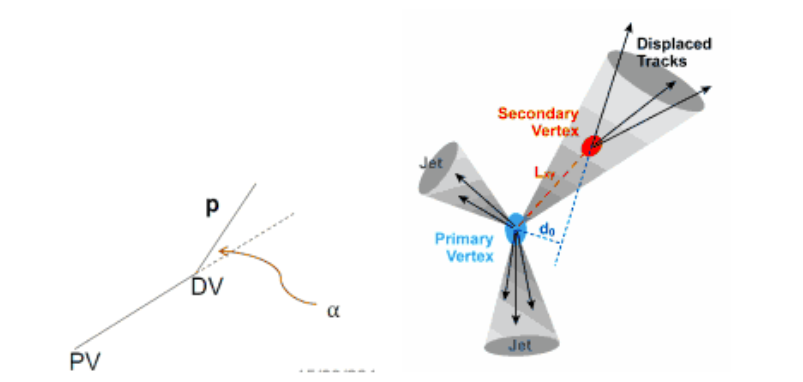
\includegraphics[width=0.8\textwidth]{Lmumu/figs/IPandDIRA.png}
\caption{Graphical representation of the DIRA (left) and \chisqip (right) variables.}
\label{fig:IPandDIRA}
\end{figure}
%
The variable $\chi^2_{FD}$ represents the flight distance of a particle from its origin vertex
divided by the corresponding uncertainty. The $\chi^2_{trk}$/ndf and $\chi^2_{vtx}$/ndf quantities are the $\chi^2$ 
from the fit to tracks and vertices, which are used to quantify their quality.
The \verb!GhostProb! quantity describes the probability of a track being fake.
By construction, cutting at a value of $k$, removes $(1 - k)\cdot 100 \%$ of fake tracks.
The \verb!hasRich!, \verb!hasCalo! and \verb!isMuon! variables are binary indicators that
the information from the RICH, calorimeter and muon detectors is available for the track.
Loose PID requirements on the proton are also applied in the pre-selection.
Details about PID quality estimators are given in Sec.~\ref{sec:PID_perf}.
%To quantify the probability of particular particle identity a combined likelihood is calculated
%combining information from the calorimeters, the RICH and the Muon detectors.
%The pion hypothesis is used as a reference point and the probability of a specific ID is given
%in terms of the difference between the Log-Likelihood of the given hypothesis and the pion.
%This variable is called is called Delta Log-Likelihood (DLL) and denoted with \verb!PID!.
%For example:
%\begin{equation}
%\verb!PID!_K = \text{DLL}_{K-\pi} = \log(\mathcal{L}_K) - \log(\mathcal{L}_\pi)
%\end{equation}
%quantifies the probability of a particle being a kaon rather than a pion.
%For details about the definition of the variables used see Ref. \cite{Loki_twiki}.
A large mass window around the \Lb peak is used to allow a fit to the sideband to be performed 
and to use sideband candidates to train a multivariate classifier.
Rare candidates are selected by the \qsq region requirements described in Sec.~\ref{sec:Lb_q2choice},
while resonant candidates are further constrained to have dimuon invariant masses
in a 100~\mevcc~interval around the known \jpsi mass~\cite{PDG2014}.

\begin{table}[h]
\centering
      \begin{tabular}{$l^c}
      \rowstyle{\bfseries}
Particle     			&  	Requirement          \\ \hline
\multirow{5}{*}{\Lb}            	&  	$4.6 < m(p\pi\mu\mu) < 7.0$ \gevcc \\
            				& 	\texttt{DIRA}$>0.9999$          \\
					& 	\chisqip$<16.0$               \\
            				& 	$\chisq_{\rm FD}>121.0$             \\
            				& 	$\chisq_{vtx}$/ndf$<8.0$          \\ \hline
\multirow{3}{*}{\Lz}      	& 	$\chisq_{vtx}$/ndf$<30.0(25.0)$              \\
         				& 	Decay time $>2$ ps              \\
					& 	$|m(p\pi)-m^{\rm PDG}_\Lz|< 35(64)$ \gevc        \\ \hline
\multirow{3}{*}{$p$/$\pi$}	& 	$p>2$ \gevc           \\ 
					& 	$\pt>250$ \mevc           \\  
            				& 	\chisqip$>9(4)$              \\ \hline
\multirow{2}{*}{$p$ (only long cand.) } 	&   	\verb!hasRICH!    \\
					&   	\verb!PID!p$> -5$  \\  \hline
\multirow{5}{*}{$\mu$}       &   	\verb!isMuon!    \\
					& 	$\chi^2_{trk}$/ndf$< 5$ 		\\
					& 	\verb!GhostProb!$<0.4$	\\
            				& 	\verb!PID!$\mu>-3$		\\
            				& 	\chisqip$>9.0$        \\      \hline
\multirow{2}{*}{Dimuon}     & 	$\chi^2_{vtx}$/ndf$<12.0$          \\
            				&	$m(\mu\mu)<7.1$~\gevcc         \\ \hline
      \end{tabular}
\caption{Summary of pre-selection requirements. Where two values are given,
the main one applies to long candidates and the one in parenthesis to downstream candidates.}
\label{tab:Lb_stripping}
\end{table}


\subsection{Neural Networks}
\label{sec:Lb_mva}

The final selection is performed using a neural network (NN) classifier based on the NeuroBayes 
package~\cite{Feindt:2006pm,feindt-2004}. The input to the neural network consists of 14 variables carrying 
information about the kinematics of the decay, the quality of tracks and vertices and the PID of the muons.
The list of the 10 most significant inputs is reported in Tab.~\ref{tab:Lb_nnInputs}, together with information 
about the importance of each input.
%
%In appendix \ref{app:MC_data_comp} we report comparisons between the variable used in data and Monte Carlo.
%On data we extract the signal distribution using the sideband subtraction technique.
%
%Under ``adds" is shown how much discriminating power a variable adds with respect to the previous ones.
%Under ``only this" is shown how much power each single input has independently of all others. Under ``loss" 
%is provided information about how much power is lost if each single input is removed.
%
Variables related to \Lz and its daughters are considered as different inputs depending on the
candidate type (long or downstream). This effectively corresponds to making a separate
training for the two categories. 
%Further details on the definition and calculation of the
%variables importance is available in Ref.~\cite{LHCb-ANA-2011-094}.
%The graphical representation of the correlation matrix is shown in Fig.~\ref{fig:Lb_nnCorrelation},
%where the variable with ID$ = 1$ is the neural network output and the IDs of the other variables are 
%listed in Tab.~\ref{tab:Lb_nnInputs}.

The NN is trained using representative samples of signal and background.  A sample of simulated 
$\Lb\to\Lz\mumu$ events is used as a proxy for the signal, while for the background a representative sample
is given by candidates in the upper $m(p\pi\mu\mu)$ invariant mass sideband. Only the upper sideband,
$m(p\pi\mu\mu) > 6 \gevcc$, is used since it contains only combinatorial background,
while the lower sideband may contain partially reconstructed and misreconstructed candidates.
In the \qsq spectrum of background samples the \jpsi and \psitwos peaks are still present indicating that charmonium
resonances are often combined with other random tracks. These candidates do not give a good description of purely
combinatorial background and, in order to avoid biases, they are removed from the training
sample by rejecting events in a 100~\mevcc~interval around the nominal \jpsi and \psitwos masses~\cite{PDG2014}.
%The events above $6 \gevcc$ used for training are not used in the subsequent analysis. 
%For the signal the training is performed combining simulated $\Lb\to\Lz\mumu$ events corresponding 
%to the beam conditions in both years. %Only triggered events are used for training.
A total of 30000 total events is used for the training from each sample. This corresponds $\sim 50\%$ of the available
sideband data sample and $\sim 20\%$ of the simulated sample. The full simulated sample is not used
as the same sample will also be used to study efficiencies. For reproducibility the events are sampled uniformly.

The single most important variable used for downstream candidates is the transverse momentum of
\Lz, which allows to reject random combination of tracks as these have preferentially low \pt.
For long candidates instead the best variable is the $\chi^2$ from a kinematic fit that constrains
the decay products of the \Lb, the \Lz and the dimuon, to originate from their respective vertices
performed using the \verb!DecayTreeFitter! tool (see Sec.~\ref{sec:DTF}).
Other variables that contribute significantly are the \chisqip of \Lb, \Lz and muons,
the separation between the \Lb and \Lz vertices and, finally, the muon PID.

Figure~\ref{fig:Lb_nnDist} shows distributions of neural network output for the signal and background samples
and purity, $P=N_{\mathrm{sig}}/N_{\mathrm{bkg}}$, as a function of the neural network output.
The distributions from test samples are also overlaid in order to check for overtraining. 
The distributions follow the same shape but with different fluctuations
indicating no significant overtraining. In general it can be concluded that the neural network
is able to separate signal from background and the training converged properly.
%
\begin{table}
\centering
\caption{Summary of the 10 most significant inputs to the neural network in order of importance.
%Column ``ID'' lists the indices used for the correlation matrix in Fig.~\ref{fig:Lb_nnCorrelation}.
Column ``adds'' gives the significance added by a given input when it is added to the list of those
ranked above. Column ``only this'' provides the power of a given input alone and ``loss'' shows 
how much information is lost when removing only a given input.}
\begin{tabular}{$l^c^c^c}
\rowstyle{\bfseries}
Input                     			& adds 		& only this & loss \\ \hline
\Lz$_{\rm DD}$ \pt                  		& 143.11 		& 143.11 	& 29.20  \\
$\chi^2_{\rm DTF}$       		& 77.81 		& 134.00 	& 51.10  \\
min(\chisqip $\mu$)             	& 61.31 		& 113.62 	& 29.76  \\
\chisqip \Lb                    		& 52.94 		& 113.23 	& 40.98  \\
\chisqip $\pi_{\rm LL}$              	& 20.29 		& 60.72 	& 12.82  \\
min(PID $\mu$)                   	& 17.91 		& 59.11 	& 13.44  \\
$\tau_{\Lb}$       		        	& 16.24 		& 35.36 	& 11.24  \\
\Lb \verb!DIRA!                         	& 12.28 		& 73.96 	& 9.98 	 \\
\Lz$_{\rm DD}$ flight distance       	& 9.47 	  	& 86.75 	& 11.24  \\
\chisqip \Lz$_{\rm DD}$              	& 10.58 		& 59.84 	& 8.88 	 \\
%Input                     			& ID  & adds 		& only this & loss \\ \hline
%\Lz$_{DD}$ \pt                  		& 15 	& 143.11 		& 143.11 	& 29.20  \\
%$\chi^2_{\rm DTF}$       		& 2 	& 77.81 		& 134.00 	& 51.10  \\
%min(\chisqip $\mu$)             	& 7 	& 61.31 		& 113.62 	& 29.76  \\
%\chisqip \Lb                    		& 5 	& 52.94 		& 113.23 	& 40.98  \\
%\chisqip $\pi_{LL}$             	& 16 	& 20.29 		& 60.72 	& 12.82  \\
%min(PID $\mu$)                  	& 8 	& 17.91 		& 59.11 	& 13.44  \\
%$\tau_{\Lb}$       		        & 3 	& 16.24 		& 35.36 	& 11.24  \\
%\Lb DIRA                        		& 4 	& 12.28 		& 73.96 	& 9.98 	 \\
%\Lz$_{DD}$ flight distance      	& 14 	& 9.47 	  	& 86.75 	& 11.24  \\
%\chisqip \Lz$_{DD}$             	& 13 	& 10.58 		& 59.84 	& 8.88 	 \\
%max(\chisqip $\mu$)             	& 6 	& 9.51  		& 97.24 	& 8.15 	 \\
%\chisqip \Lz${}_{LL}$           	& 10 	& 7.31 		& 54.27 	& 10.32  \\
%max(PID $\mu$)                  	& 9 	& 6.99 		& 69.33 	& 6.87 	 \\
%$\pi_{LL}$ \pt                  		& 18 	& 6.13 		& 47.03 	& 7.12 	 \\
%\Lz${}_{LL}$ \pt         	    		& 12 	& 5.58 		& 49.64 	& 5.86 	 \\
%\chisqip $p_{LL}$               	& 17 	& 4.48 		& 53.01 	& 4.18 	 \\
%\chisqip $p_{DD}$               	& 20 	& 3.43 		& 55.09 	& 3.31 	 \\
%\Lz$_{LL}$ flight distance     	& 11 	& 0.87 		& 52.52 	& 0.86 	 \\
%$p_{DD}$ \pt                    		& 21 	& 0.74 		& 129.58 	& 0.75 	 \\
%\chisqip $\pi_{DD}$             	& 19 	& 0.24 		& 70.43 	& 0.24 	 \\
\hline
\end{tabular}
\label{tab:Lb_nnInputs}
\end{table}
%
%\begin{figure}
%\centering
%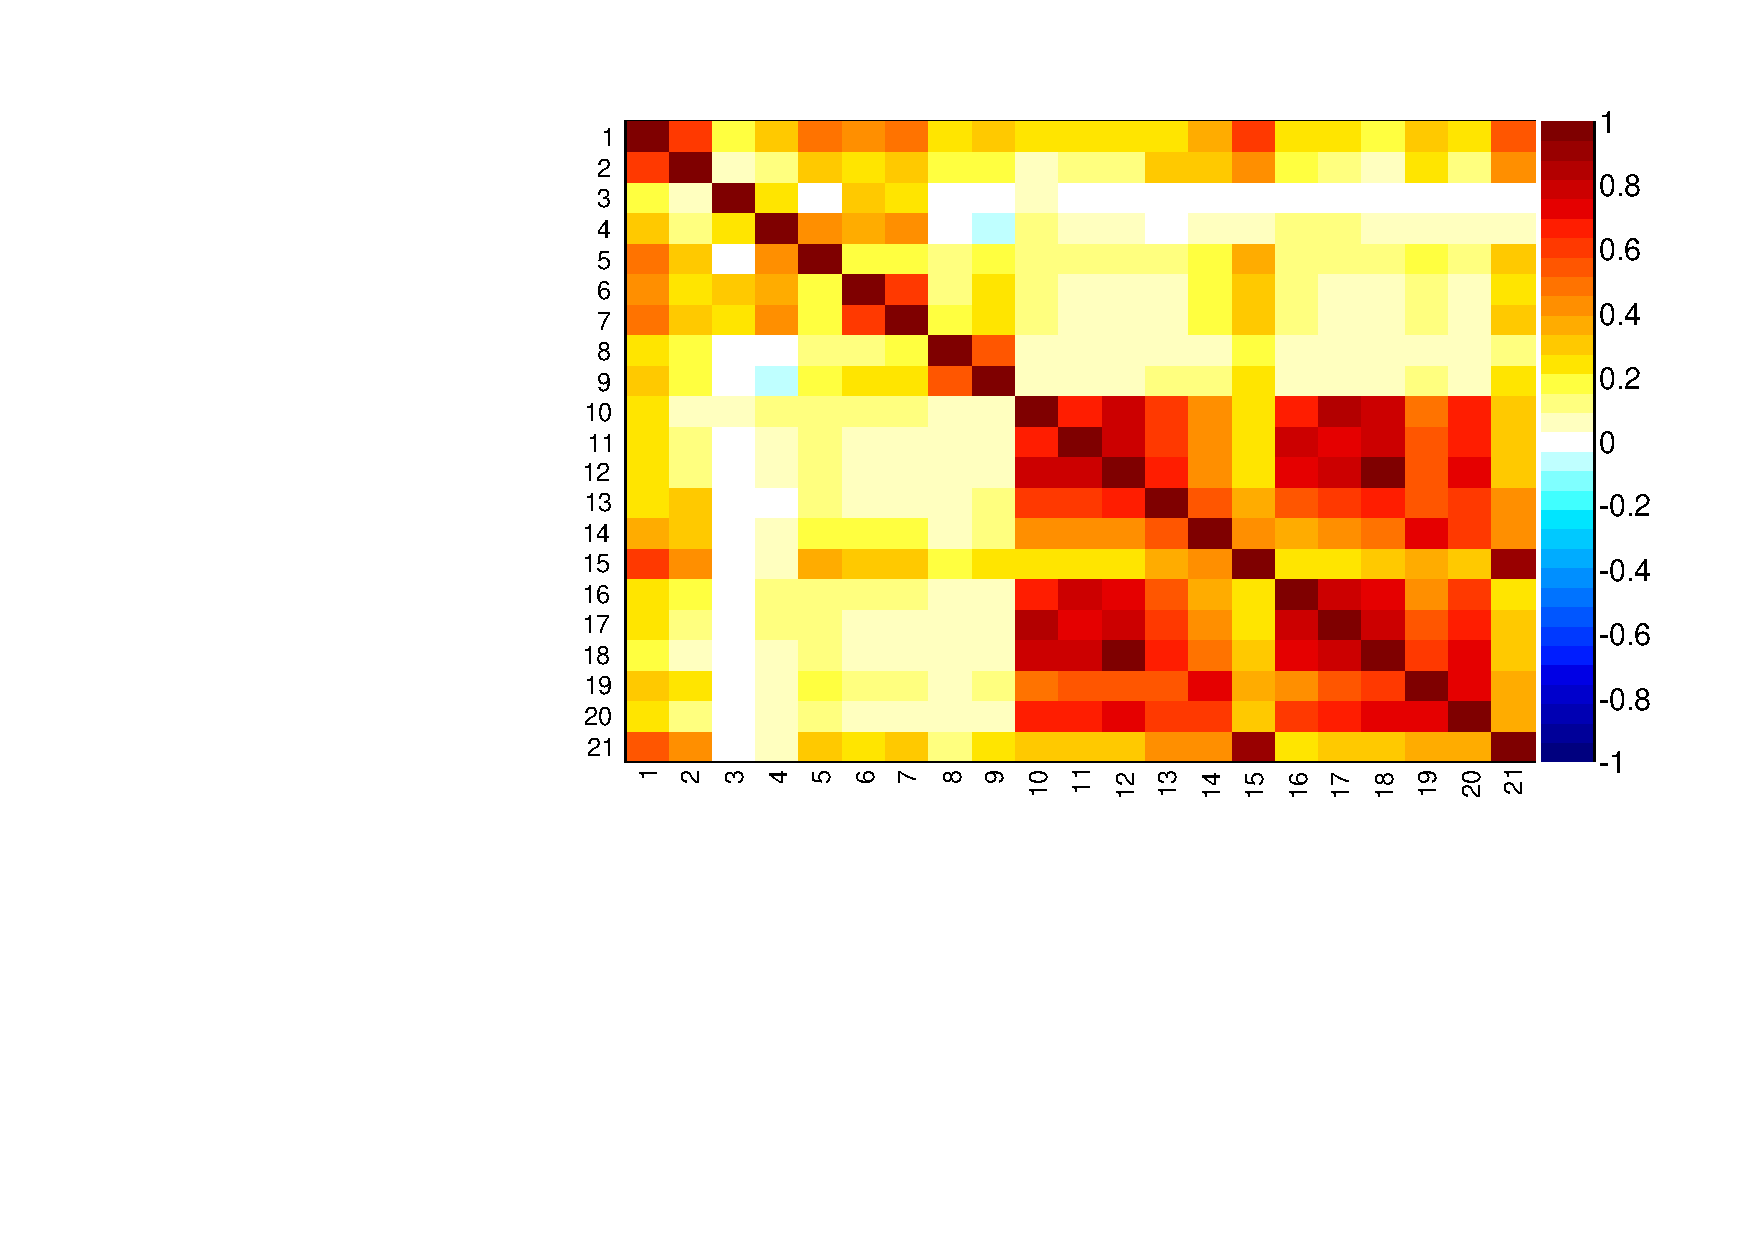
\includegraphics[width=0.7\textwidth]{Lmumu/figs/correlation.pdf}
%\caption{Graphical representation of the correlation matrix between neural network inputs.
%Column/row number 1 is the correlation to the neural network output. All
%others give the correlation between inputs with numbering scheme corresponding
%to the ID column of Tab.~\ref{tab:Lb_nnInputs}. 
%Correlation is calculated using all events without distinguishing signal and background.
%}
%\label{fig:Lb_nnCorrelation}
%\end{figure}
%
\begin{figure}
\centering
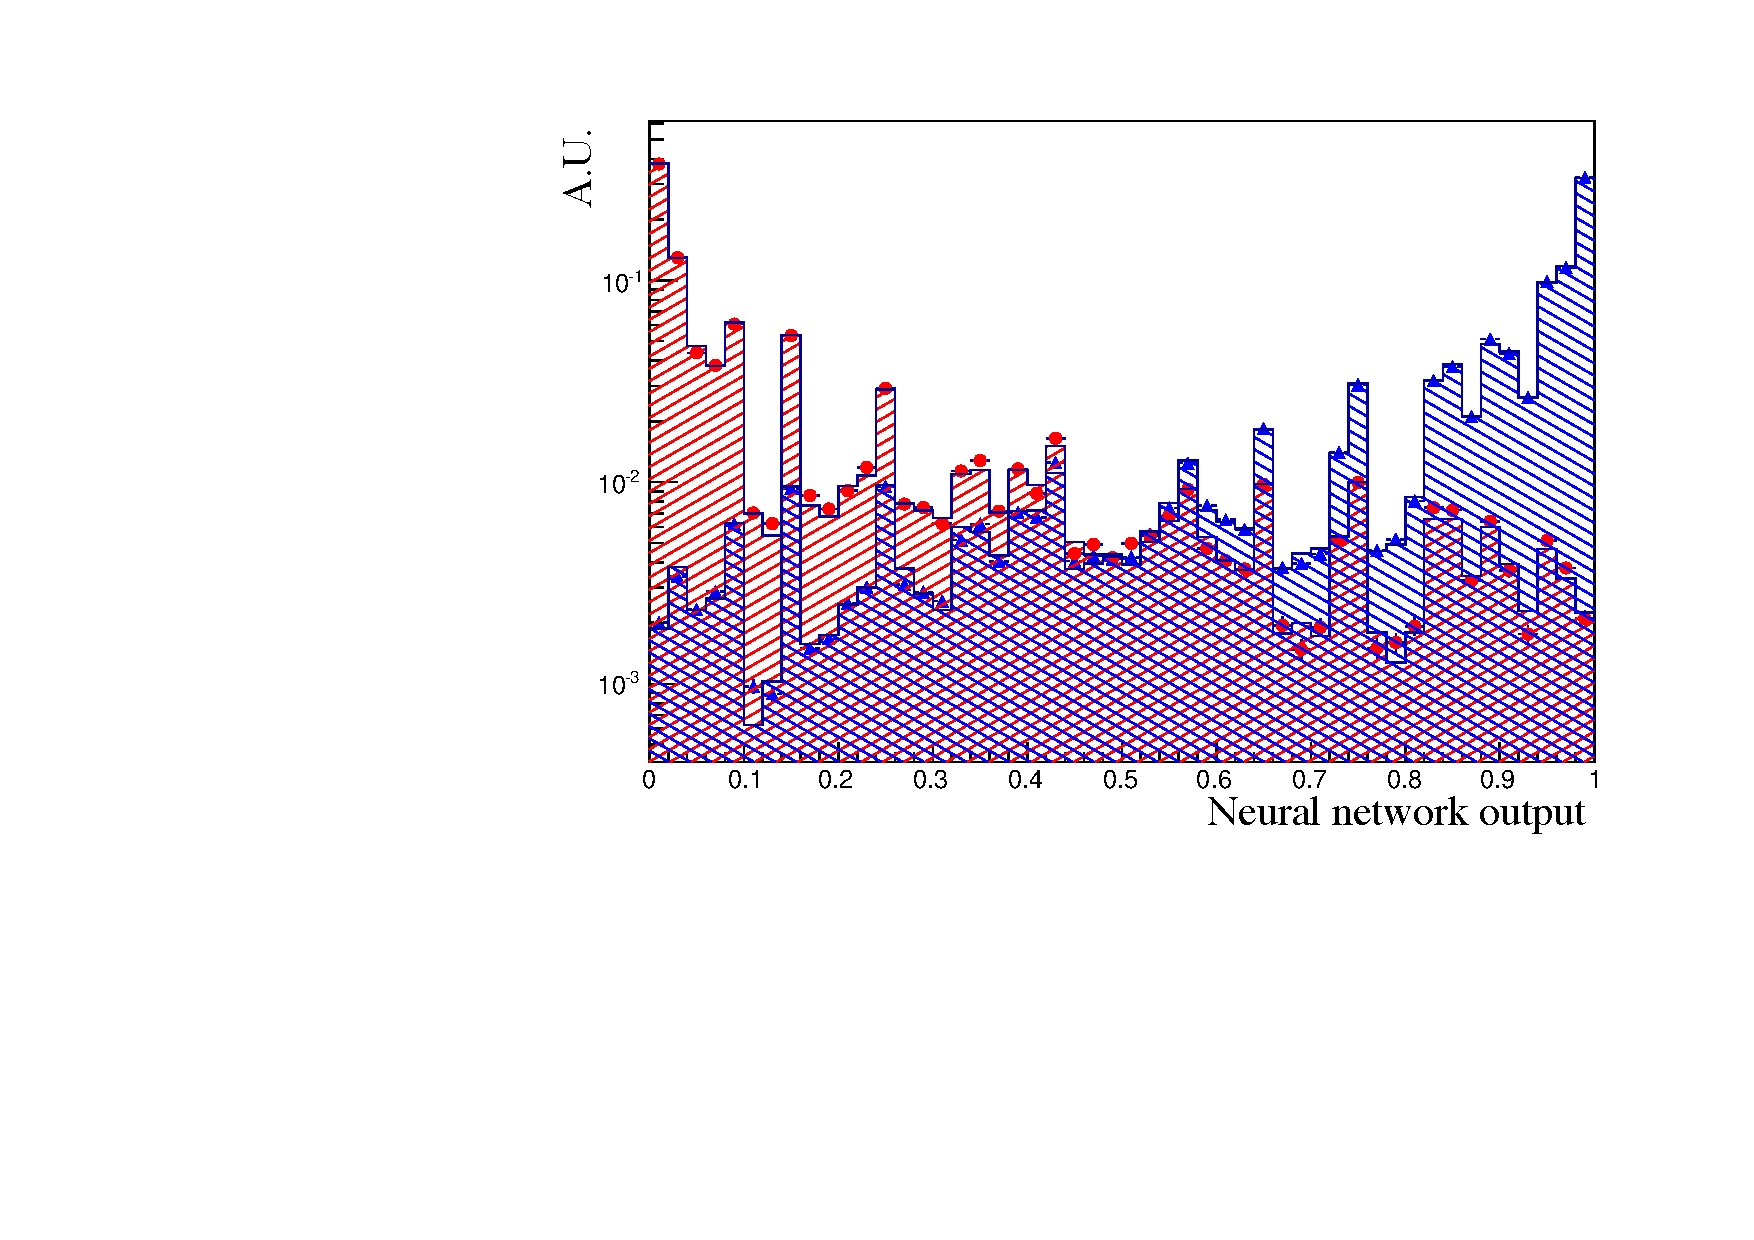
\includegraphics[width=0.49\textwidth]{Lmumu/figs/TrainAndTest.pdf}
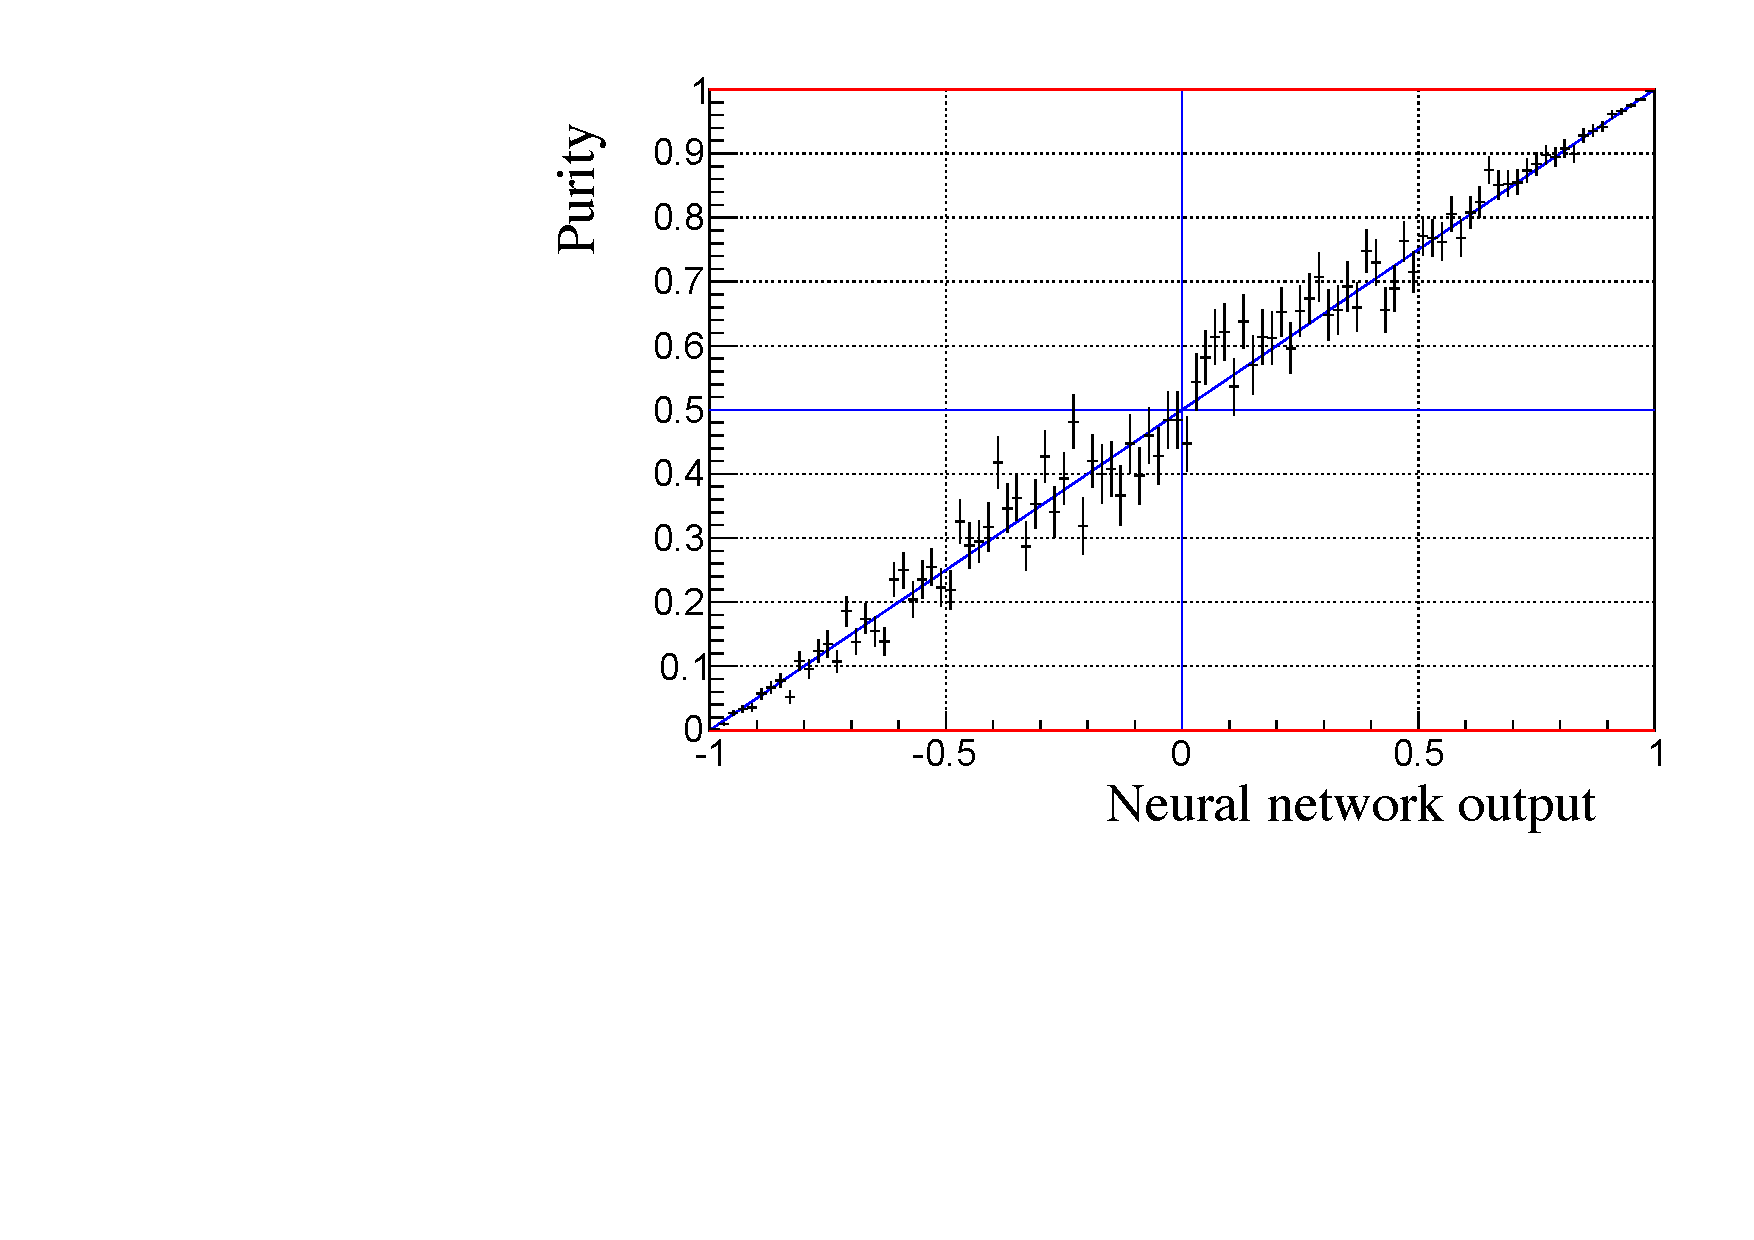
\includegraphics[width=0.49\textwidth]{Lmumu/figs/purity_NN.pdf}
\caption{(left) Neural network output distribution for training (points) and test (stripes) samples,
for signal and background events. (right) Purity as a function of neural network output.}
\label{fig:Lb_nnDist}
\end{figure}
%
It can happen that too much information is given to the classifier, which becomes able to 
calculate the invariant mass of the candidates from the input variables.
This can generate fake peaks and it is therefore important to check
for correlations between the 4-body invariant mass and the NN output.
Figure~\ref{fig:Lb_NNprofiles} reports the average neural network output as a function of
the 4-body $m(p\pi\mu\mu)$ invariant mass for data and simulation. The distributions
are flat indicating that no significant correlation is present.
%
\begin{figure}
\centering
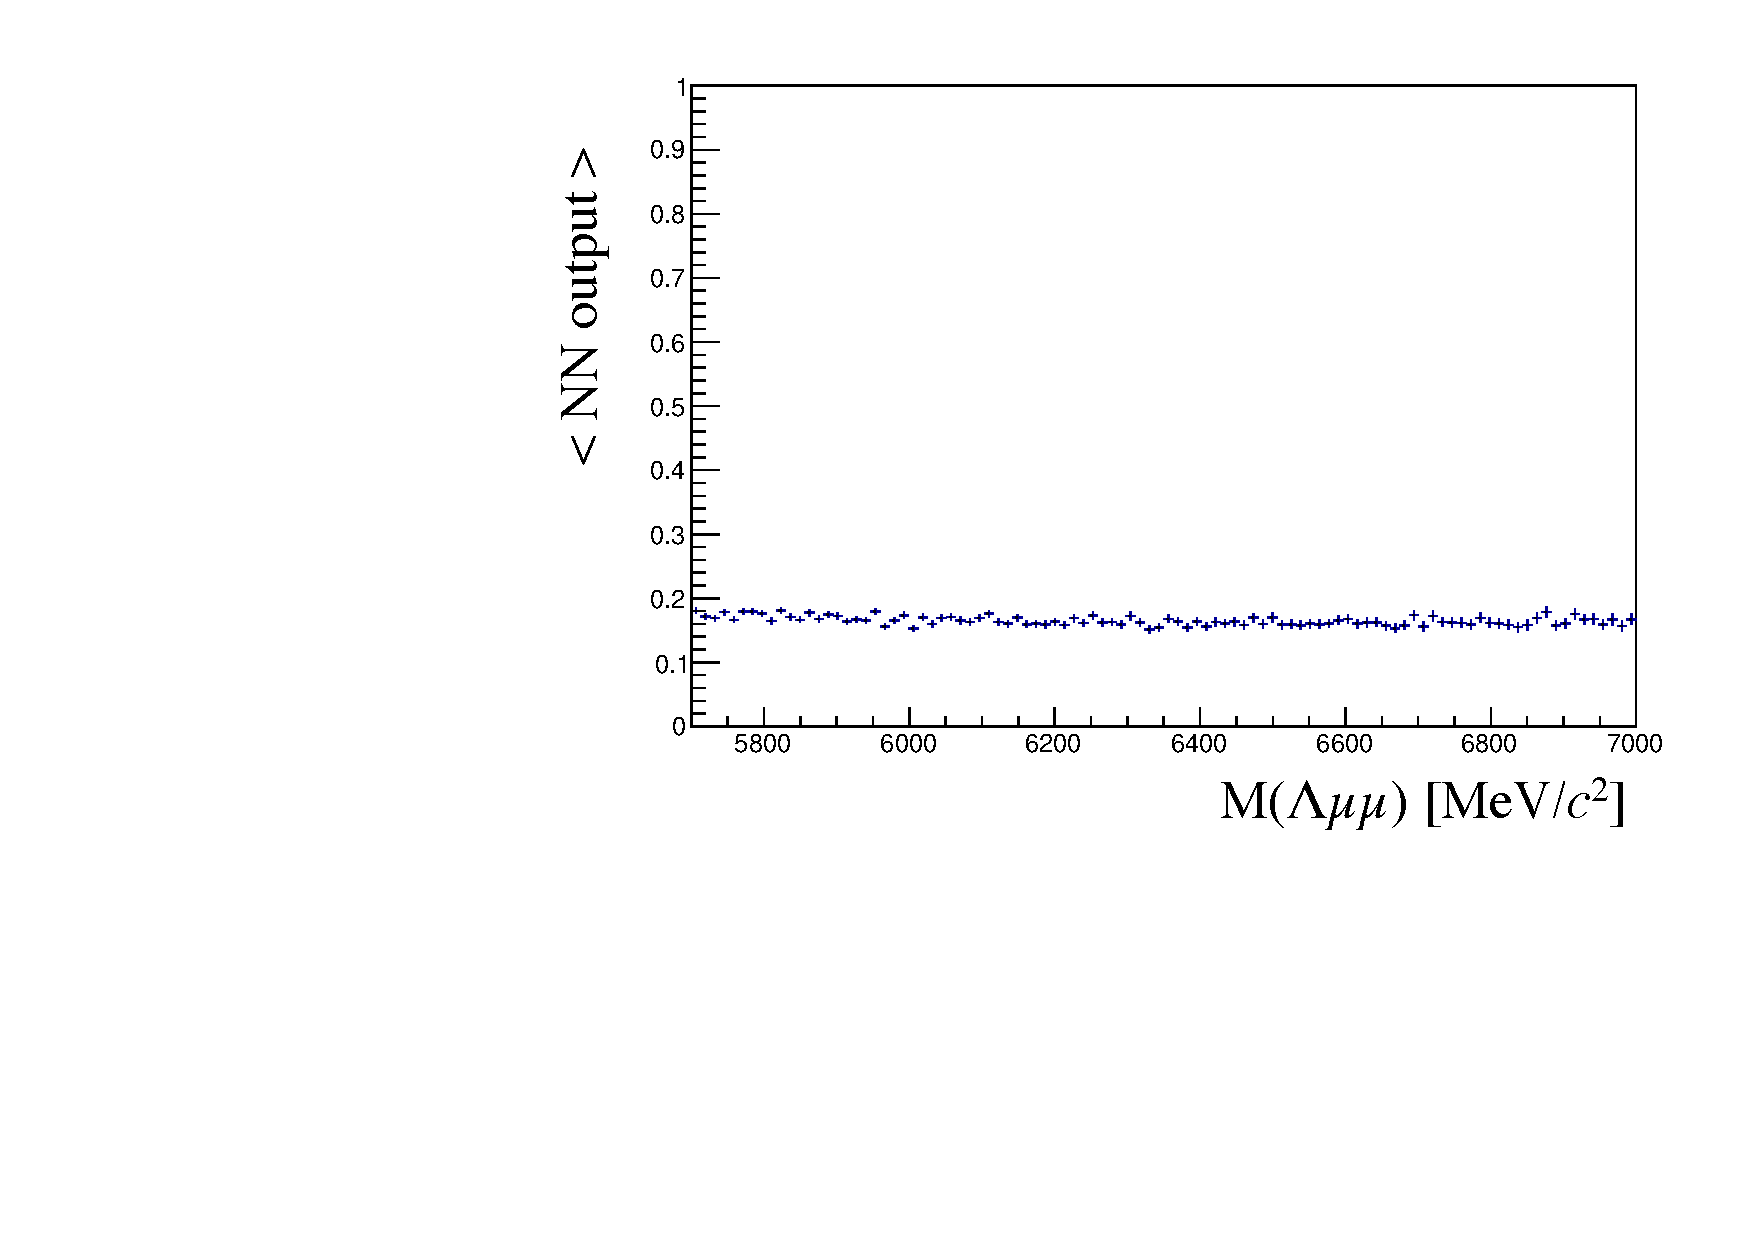
\includegraphics[width=0.49\textwidth]{Lmumu/figs/NNout_profile_vs_LbMM_bkgData.pdf}
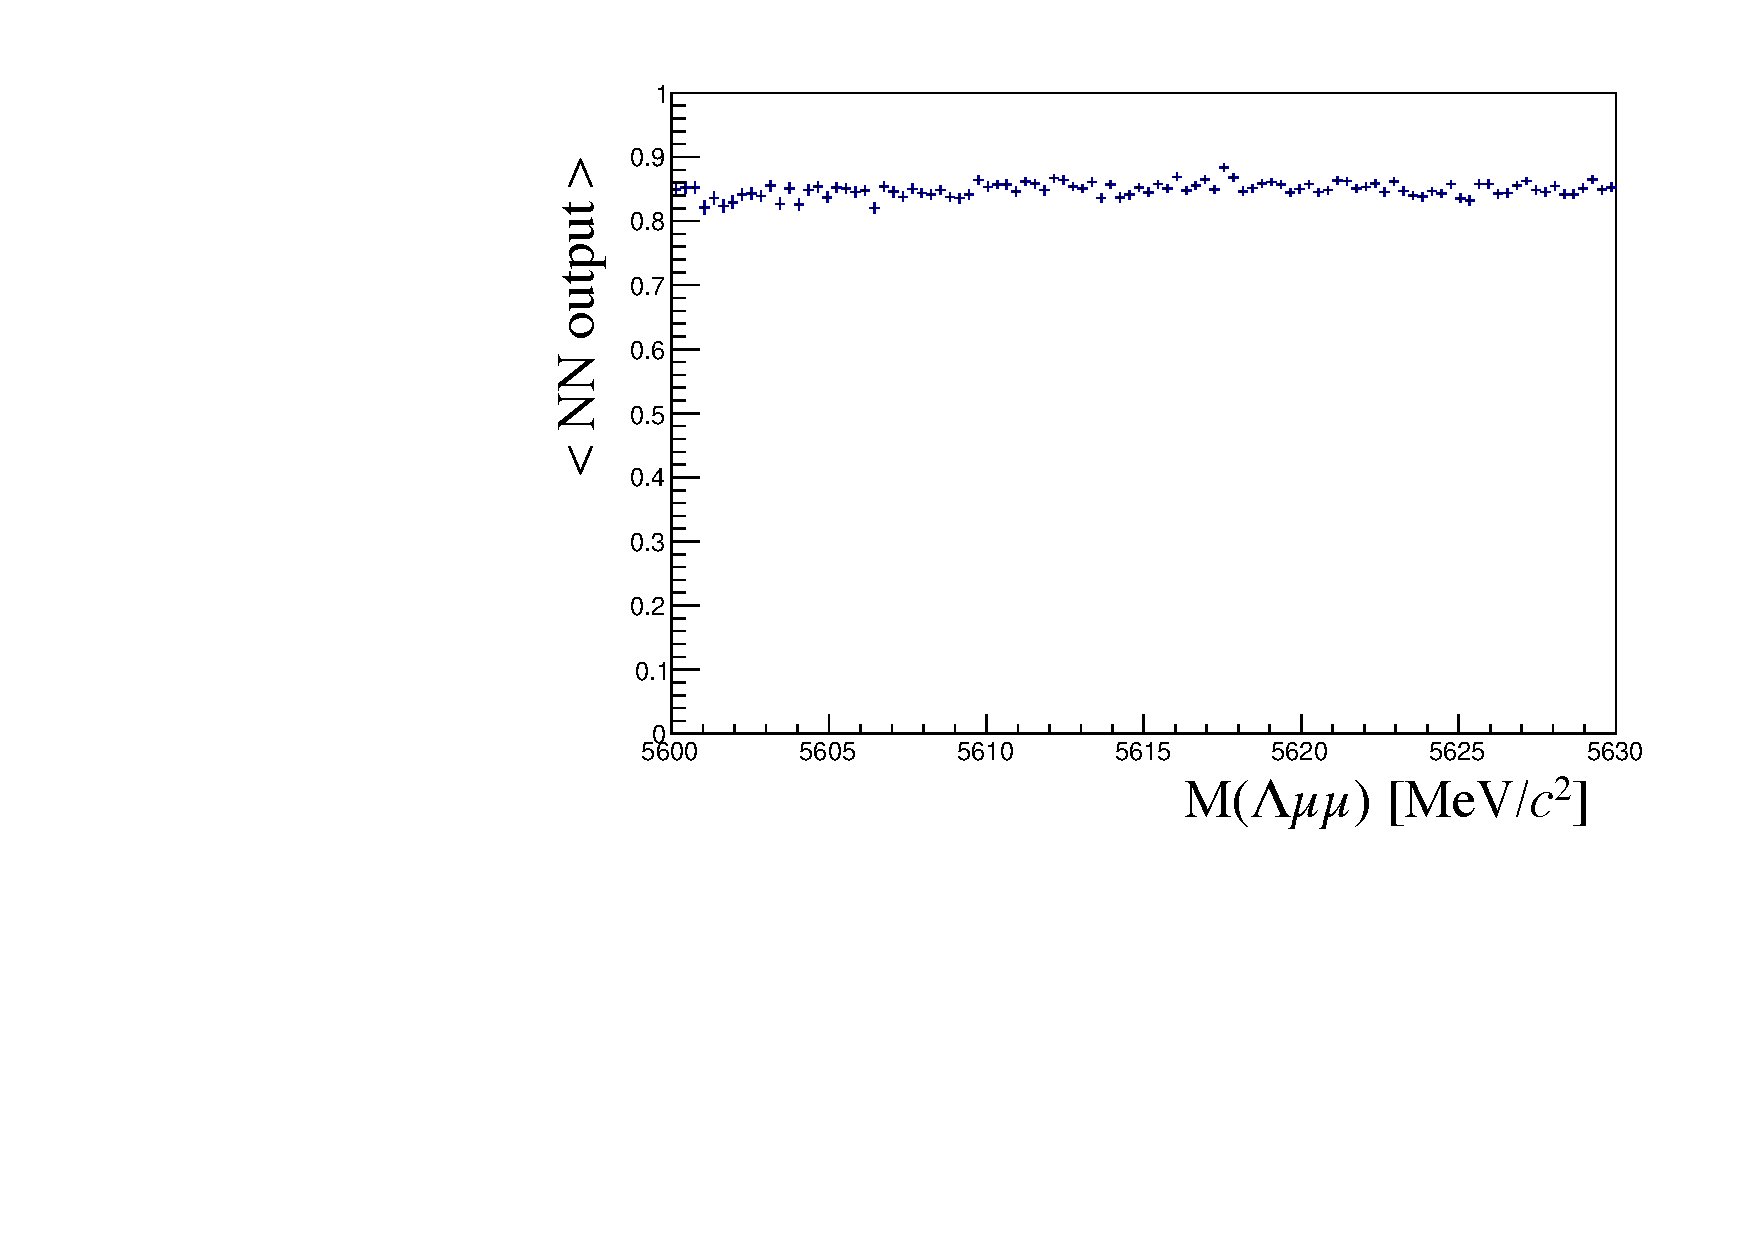
\includegraphics[width=0.49\textwidth]{Lmumu/figs/NNout_profile_vs_LbMM_MCsignal.pdf}
\caption{Average value of NN output as a function of \Lb mass for data sideband (left) and simulated signal (right) events.}
\label{fig:Lb_NNprofiles}
\end{figure}




%As side note, we do not imply any particle identification on the \Lz daughters, nor we explicitly
%veto contributions where \KS is misreconstructed as \Lz. As will be seen later, \Bz decays
%containing \KS do not pose significant issues and any sensible attempt to significantly suppress
%them would result in significant loss of the statistics.




\subsection{MVA optimisation}
\label{sec:Lb_mva_opt}

In the high \qsq region, where the signal is already observed, the requirement on the neural network output
is chosen maximising the significance, $N_{\mathrm{S}}/\sqrt{N_{\mathrm{S}}+N_{\mathrm{B}}}$, where
$N_\mathrm{S}$ and $N_\mathrm{B}$ are the numbers of expected signal and background candidates respectively.
$N_\mathrm{S}$ is derived from simulation but, as an arbitrary number of events can be generated, it
needs to be normalised. To do this, the invariant mass distribution of real $\Lb\to\jpsi\Lz$ candidates
is fit after pre-selection (including all requirements but MVA). This is possible as the peak of the resonant
channel is already well visible before the MVA cut. The resonant yield is then scaled by the ratio
of between the $\Lb\to\Lz\mumu$ and $\Lb\to\jpsi\Lz$ branching fractions as measured 
by LHCb on 2011 data 
\begin{equation}
\BR(\Lb\to\Lz\mumu) / \BR(\Lb\to\jpsi\Lz) =  1.54 \times 10^{-3}
\end{equation}
\noindent
and by the $\jpsi\to\mumu$ branching fraction. In summary:
\begin{equation}
N_\mathrm{S} = N_\jpsi \cdot \frac{\BR(\Lb\to\Lz\mumu)}{\BR(\Lb\to\jpsi\Lz) \cdot \BR(\jpsi\to\mumu) }.
\end{equation}
%
The number of expected background events instead is derived fitting the data
sideband with an exponential and extrapolating under the signal region.

In the low \qsq region, where the signal is unobserved, the so called ``Punzi figure-of-merit",
$N_{\mathrm{S}}/(n_\sigma/2+\sqrt{N_{\mathrm{B}}})$, is maximised~\cite{Punzi:2003bu}.
This figure-of-merit is considered to be optimal for discovery and the parameter $n_\sigma$ corresponds to
the number of expected standard deviations of significance, in this analysis $n_\sigma = 3$ is used.
Moreover, the Punzi shape does not depend on the relative normalisation between signal and background, which
is important since the signal is still unobserved at low \qsq and the existing predictions vary significantly
for this region. The dependence of the figure-of-merit for both \qsq regions is shown in Fig.~\ref{fig:Lb_FOM}, and curves
of signal efficiency versus background rejection are shown in Fig.~\ref{fig:Lb_ROC}.

For final selection the neural network output is required to be larger than 0.76 for candidates in the high \qsq region
and 0.97 for the low \qsq ones. Using these requirements the neural network retains approximately 96\% (66 \%)
of downstream candidates and 97 \% (82 \%) of long candidates for the high (low) \qsq selection, with respect to
the pre-selected samples. After full selection $\sim 0.5$\% of the events contain multiple candidates
which are randomly rejected keeping only one candidate per event. 
%
%As reminder, in low \qsq region we start with much larger background than in high \qsq region.
%Moreover, while background rejection looks similar at selected requirement, in terms of amount of background kept, there is huge difference. 
%
To normalise the branching ratio measurement \jpsi events are selected using the low and high \qsq requirements
 to normalise respectively low and high \qsq intervals. 
%
\begin{figure}
\centering
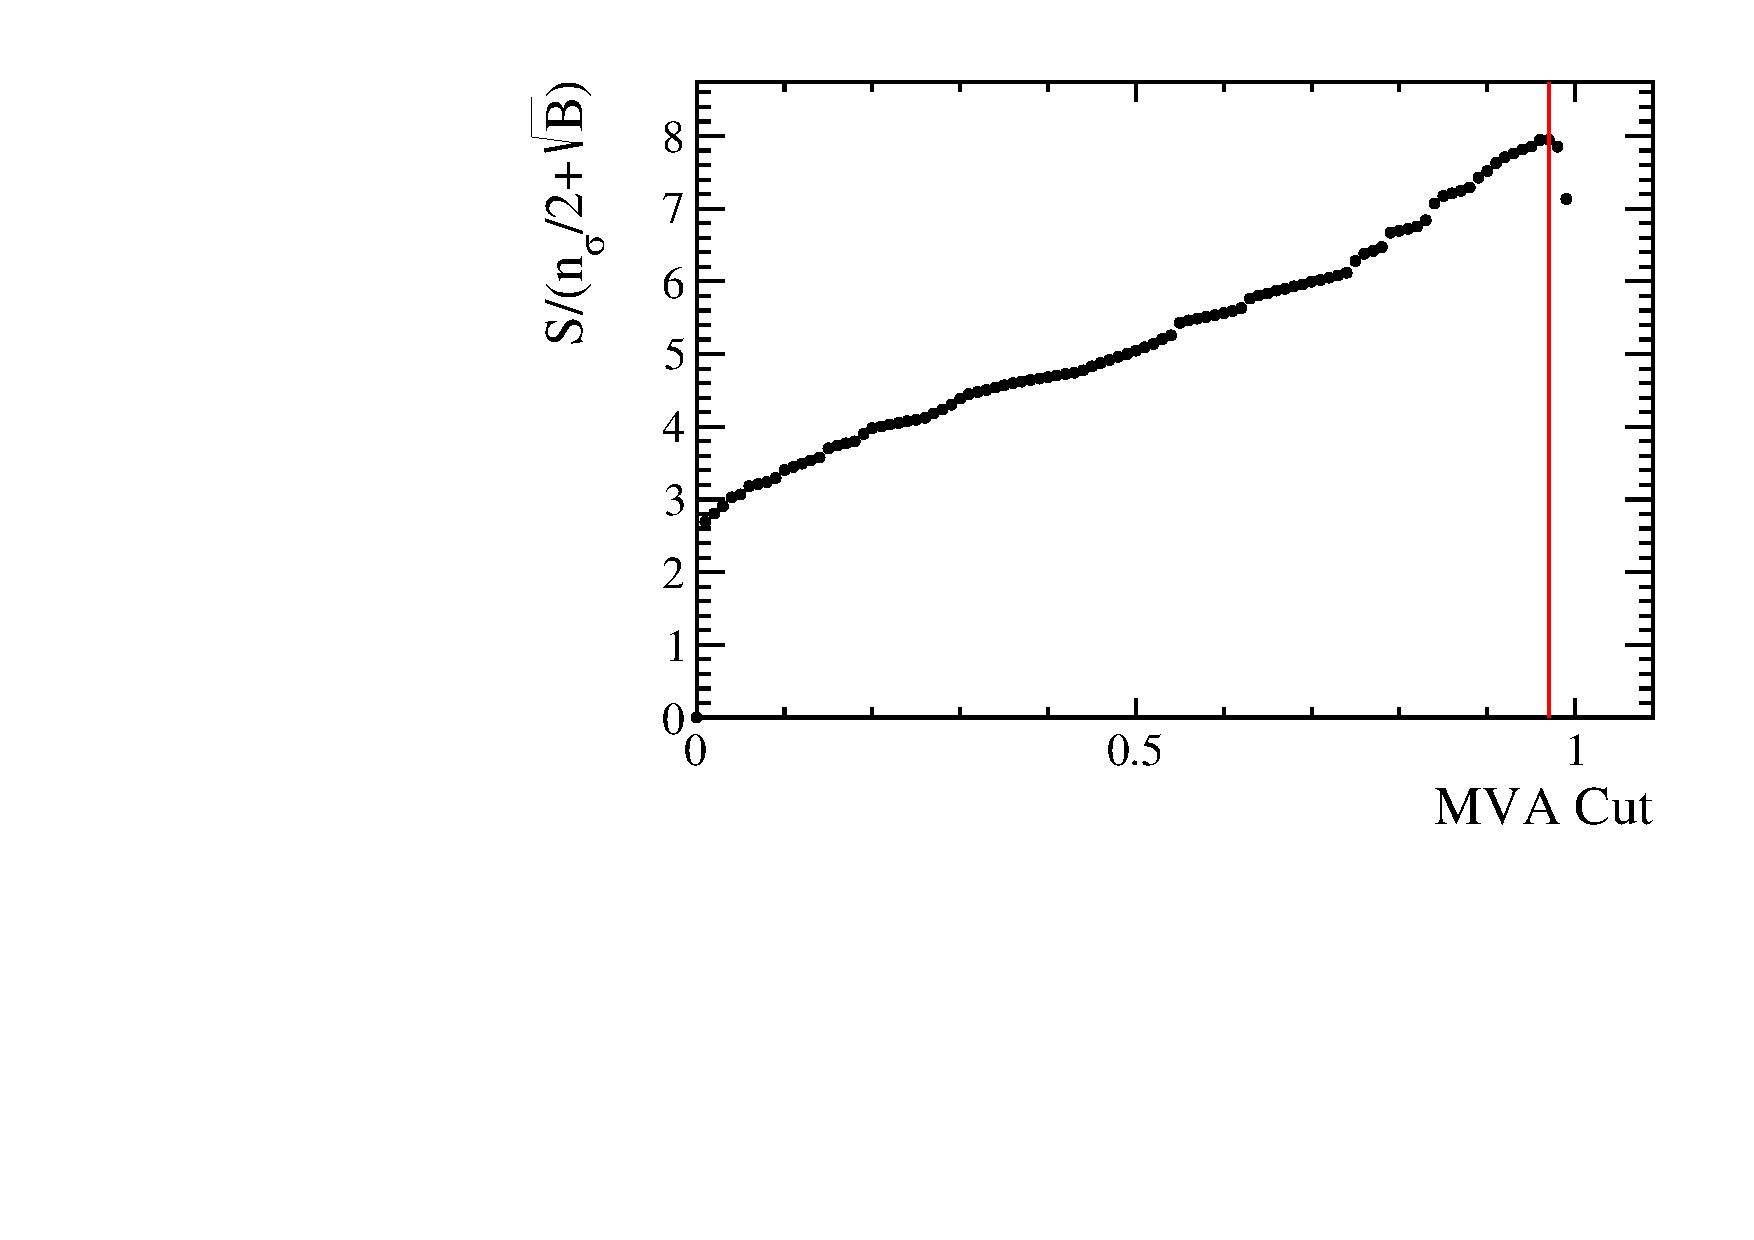
\includegraphics[width=0.49\textwidth]{Lmumu/figs/Lmumu_lowQ2_FoM.pdf}
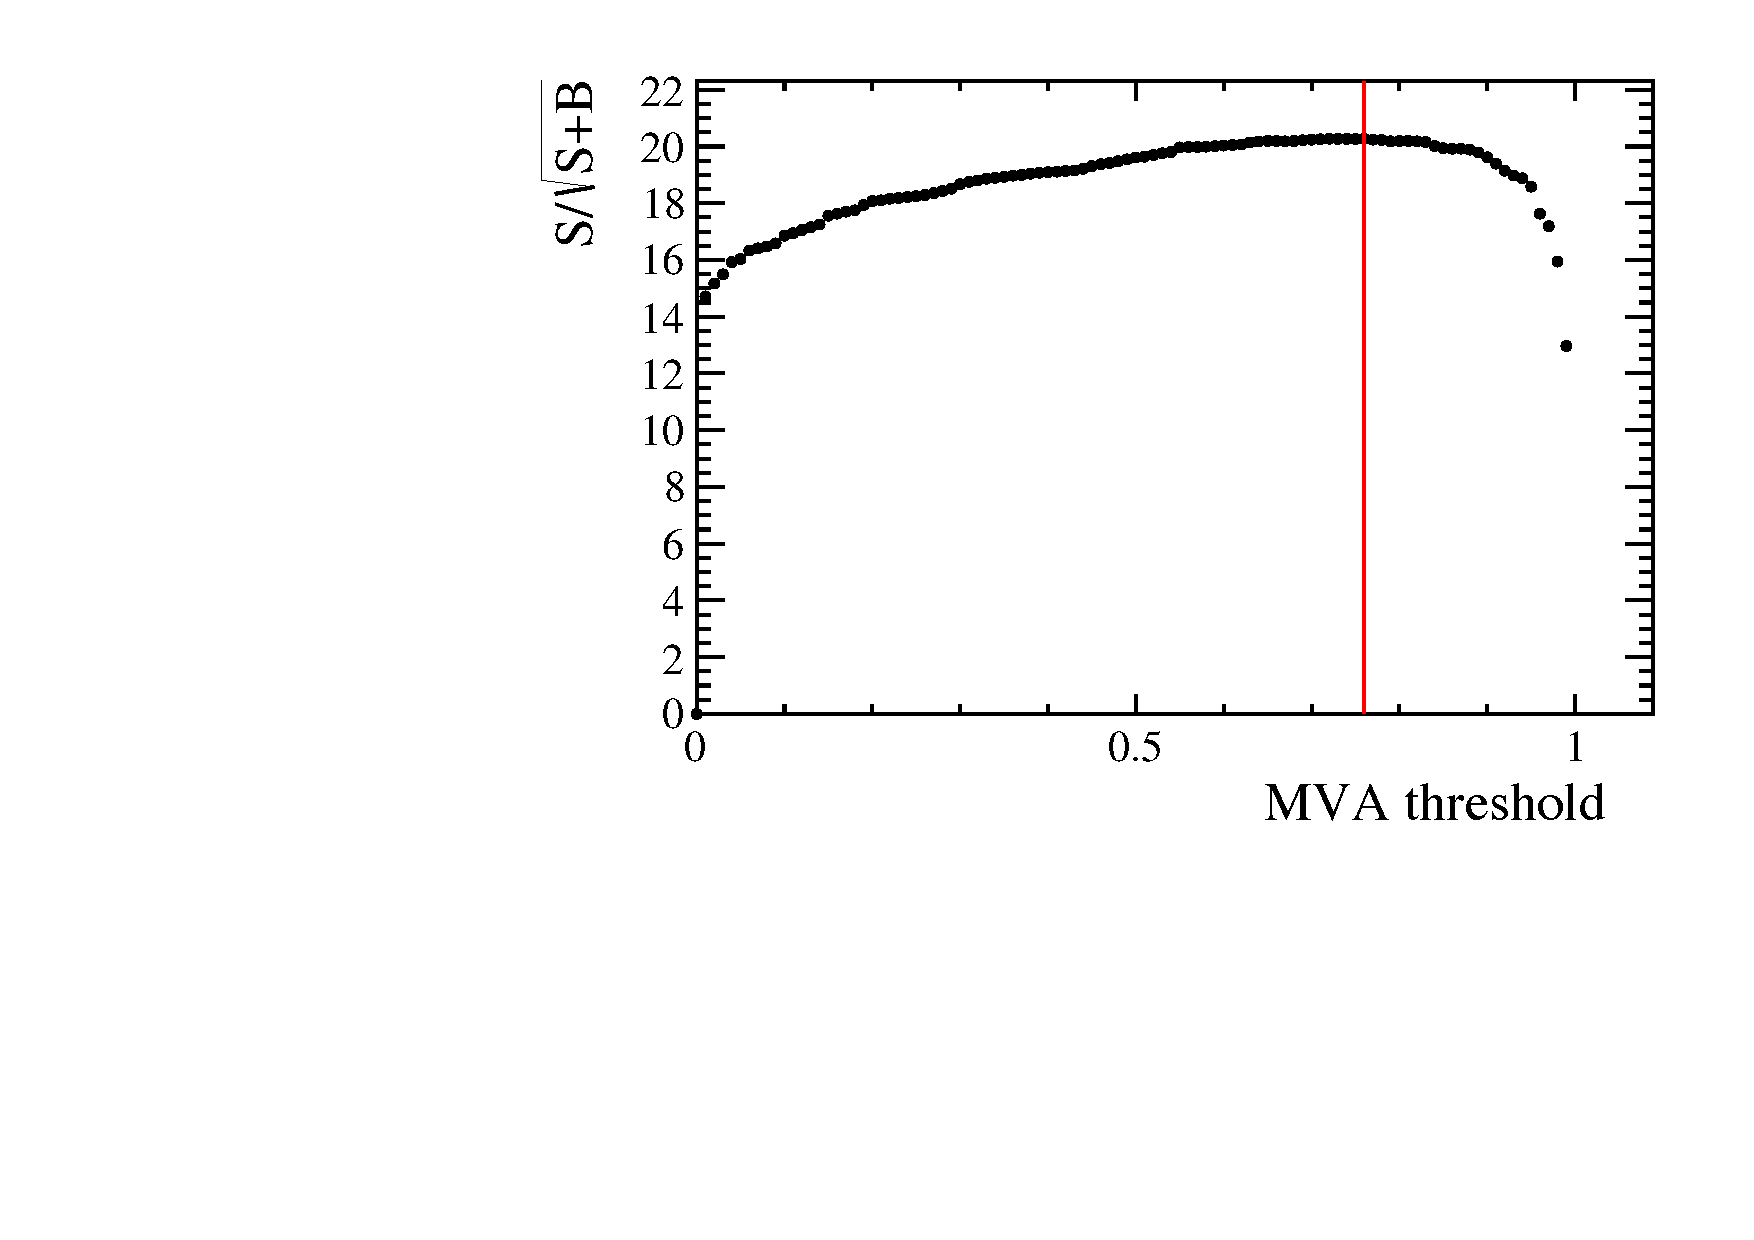
\includegraphics[width=0.49\textwidth]{Lmumu/figs/Lmumu_highQ2_FoM.pdf}
\caption{Dependence of the figure-of-merits on the neural network output requirement for the low \qsq
(left) and high \qsq (right) regions. The vertical lines correspond to the chosen cuts.}
\label{fig:Lb_FOM}
\end{figure}
%
\begin{figure}
\centering
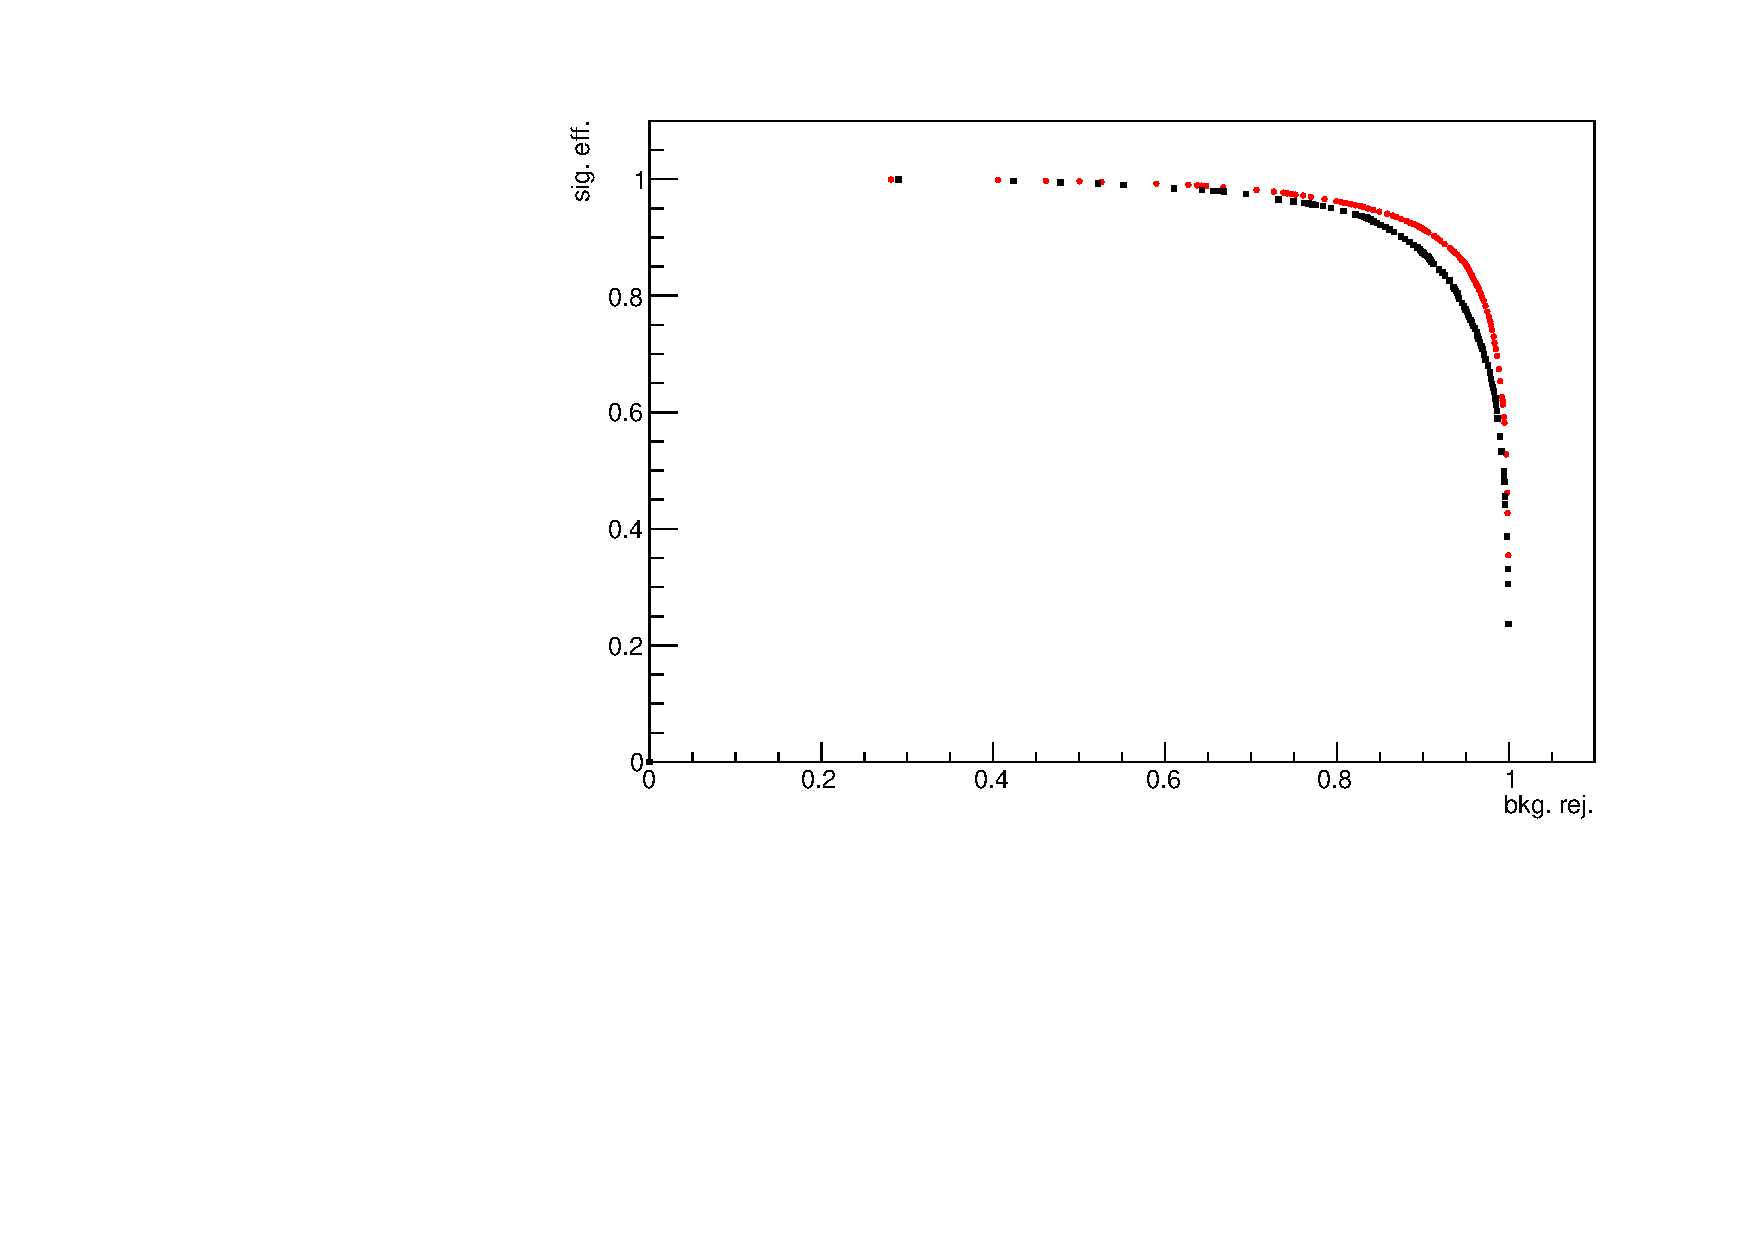
\includegraphics[width=0.7\textwidth]{Lmumu/figs/ROC.pdf}
%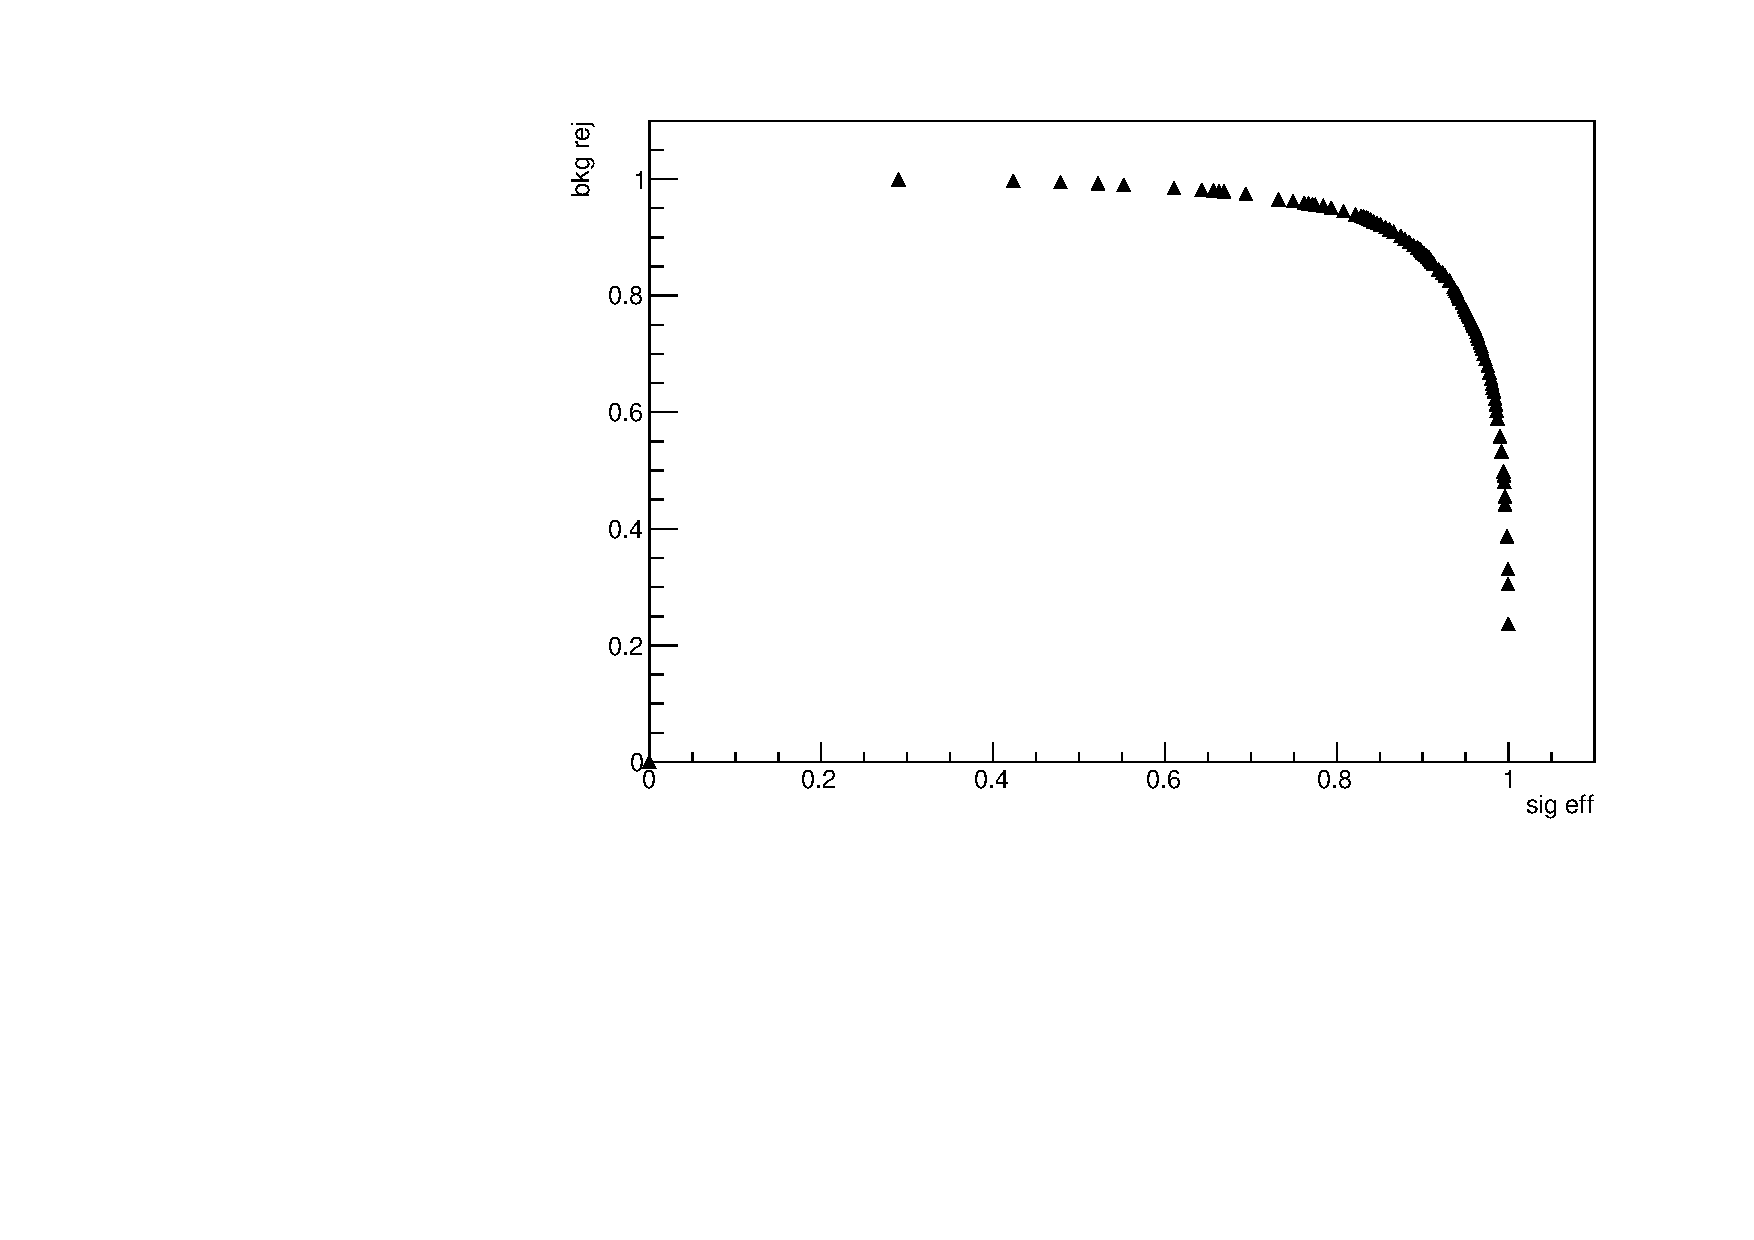
\includegraphics[width=0.48\textwidth]{Lmumu/figs/ROC_Lmumu_highQ2.pdf}
\caption{Receiver operating characteristic (ROC) curves for low \qsq (black) and high \qsq (red).
They show the signal efficiency versus the background rejection.
The optimal points on these curves are the closest ones to (1,1). }
\label{fig:Lb_ROC}
\end{figure}

%\begin{figure}
%\centering
%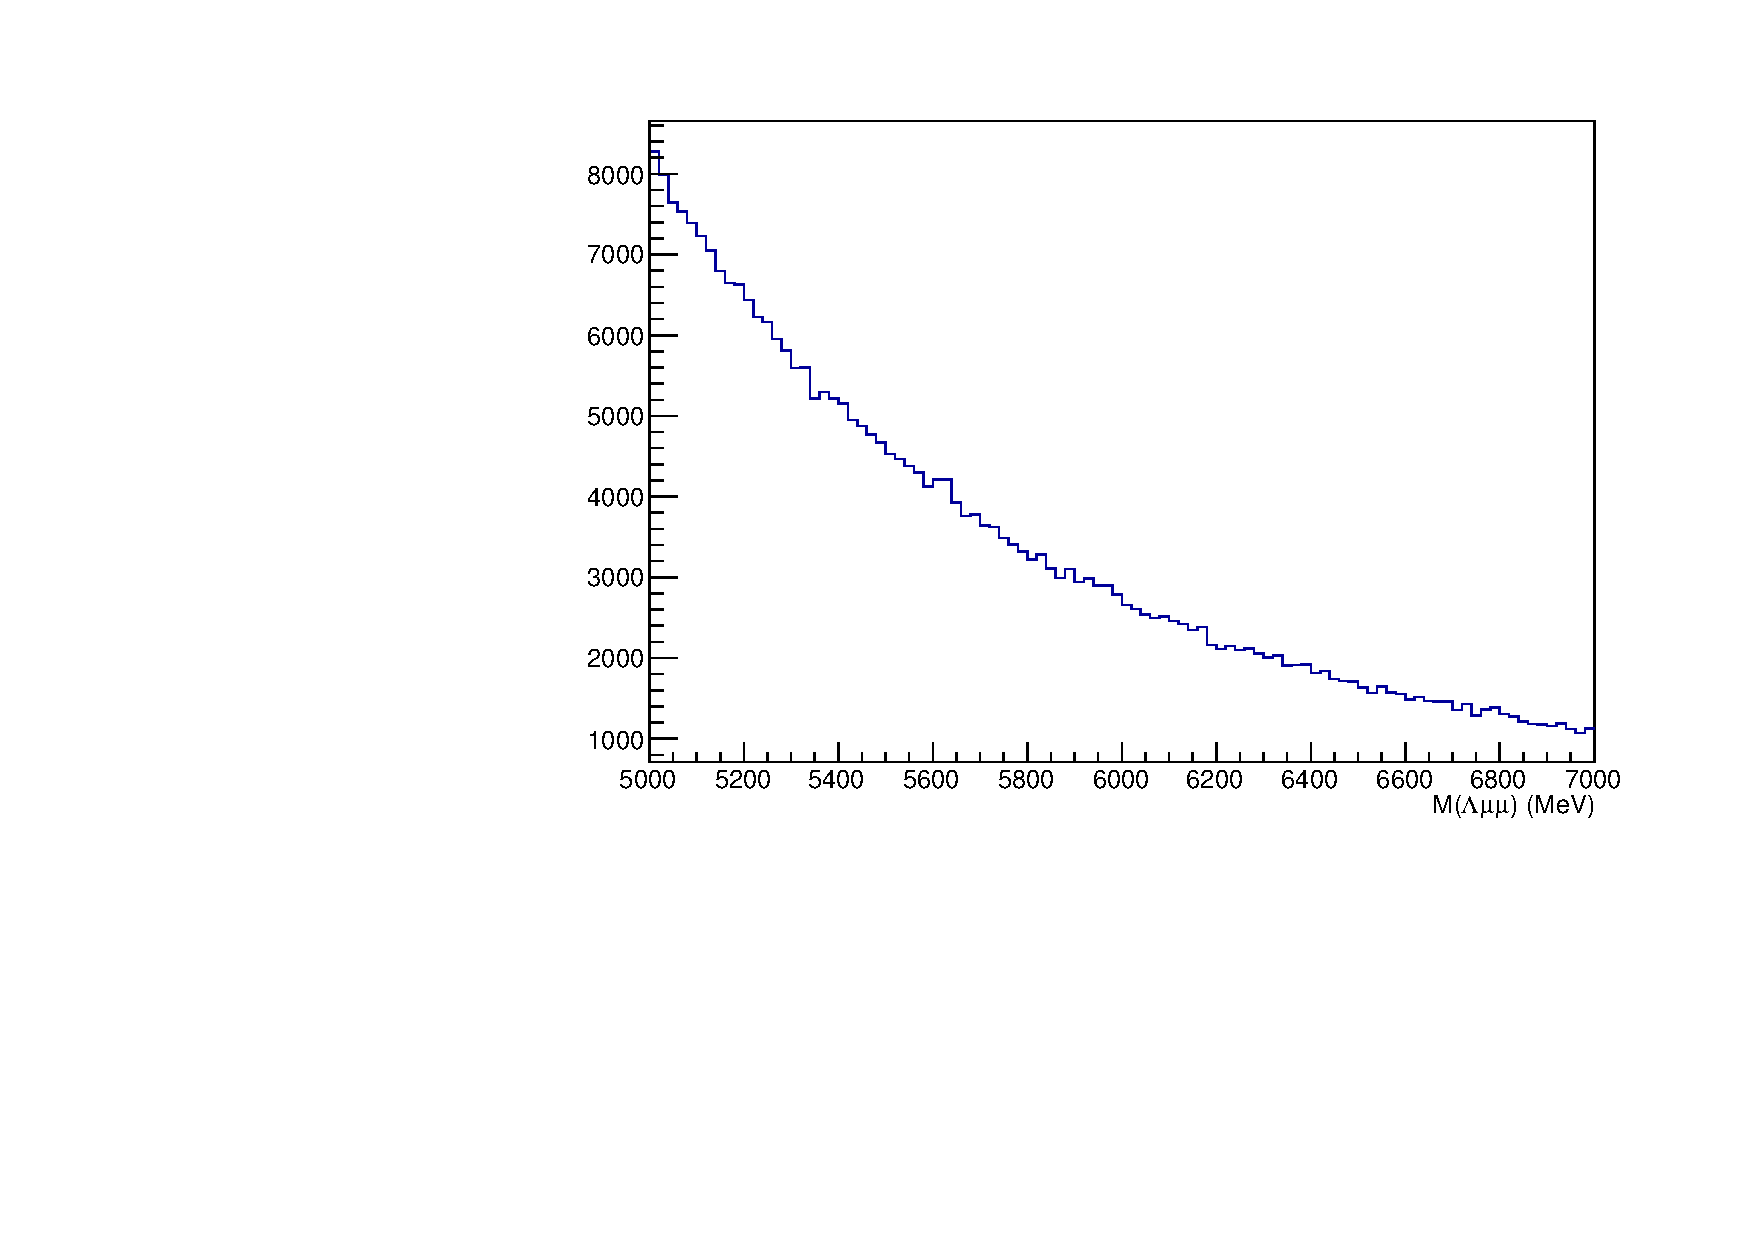
\includegraphics[width=0.48\textwidth]{Lmumu/figs/Lb_MM_beforeMVAcut.pdf}
%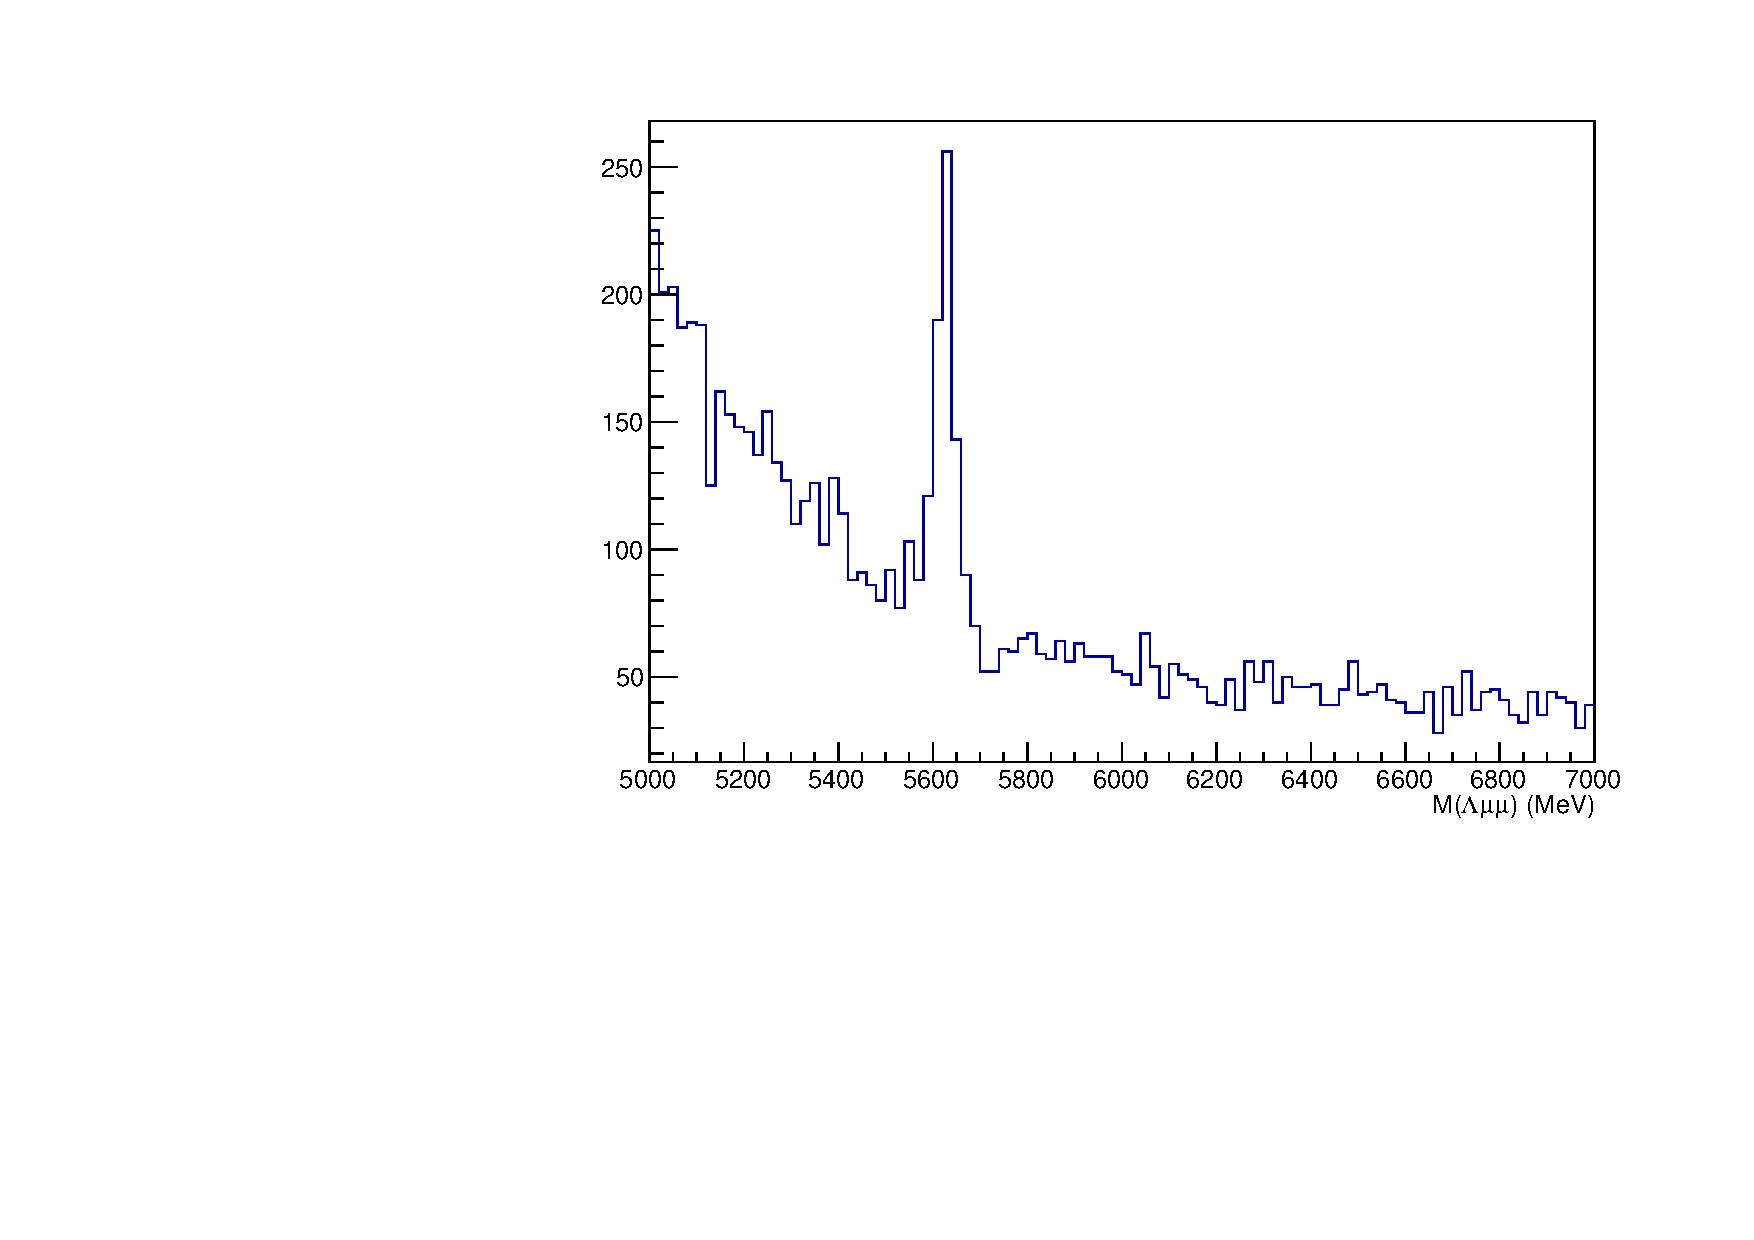
\includegraphics[width=0.48\textwidth]{Lmumu/figs/Lb_MM_afterMVAcut.pdf}
%\caption{Invariant mass distribution $\Lb\to\Lz\mumu$ candidates before the MVA cut (left) and after the cut (right). This plot includes all data
%outside charmonium vetoes.}
%\label{fig:massDists}
%\end{figure}
%
%In Fig.~\ref{fig:massDists} we show invariant mass distributions of rare decay candidates before and after the MVA selection; the plot after MVA corresponds to final selection.
%In Fig.~\ref{fig:L0mass} we show the $m(p\pi)$ invariant mass of selected candidates, peaking at the PDG value for \Lz mass (1115 \mevcc).
%This indicates that our sample is dominated by real \Lz decays.  
%
%\begin{figure}
%\centering
%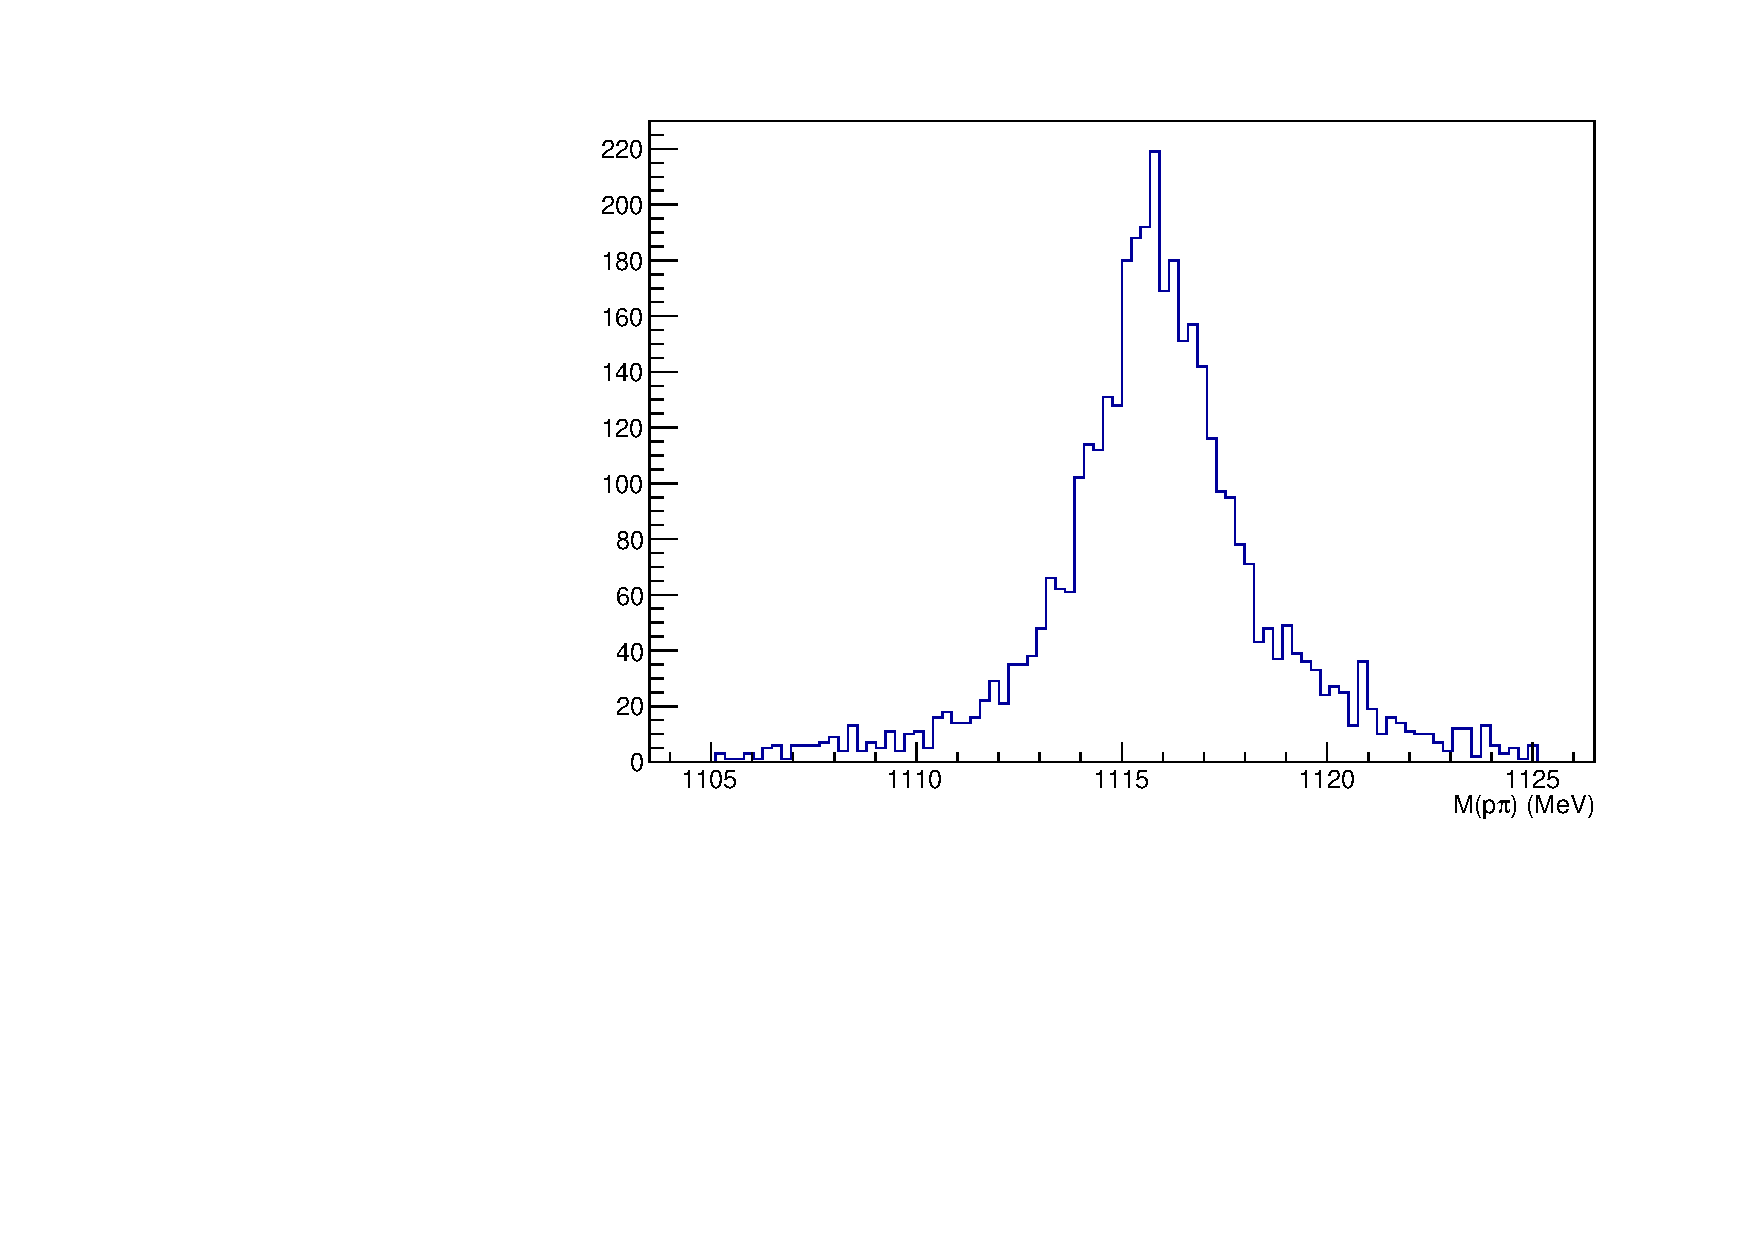
\includegraphics[width=0.7\textwidth]{Lmumu/figs/Lambda0_mass.pdf}
%\caption{Invariant mass $m(p\pi)$ of fully selected candidates.}
%\label{fig:L0mass}
%\end{figure}




\subsection{Trigger}

Finally, specific trigger lines are selected, corresponding to events triggered by muons
which formed the reconstructed candidate. This is denoted as Trigger On Signal (TOS).
The trigger lines used in the analysis are listed in Tab.~\ref{tab:Lb_triggerLines}.
The logical {\em or } of the lines on the same lever is required and the logical {\em and }
of those on different levels.
The \verb!L0Muon! trigger requires hits in the muon detector and triggers if a muon with $\pt > 1.5 \gevc$ is identified.
\verb!L0Dimuon! imposes the same requirement on the sum of the transverse momenta of two tracks.
The \verb!Hlt1TrackAllL0! performs a partial reconstruction of the events and applies basic requirements on the
IP, $\chi^2$ and \pt of tracks; it triggers if the L0 decision is confirmed. \verb!Hlt1TrackMuon! applies looser requirements 
but in addition requires the \verb!isMuon! variable (see Sec.~\ref{sec:PID_perf}) to be true to limit the yield.
Finally, at the Hlt2 level, a complete reconstruction is done and a multivariate analysis is used to identify decay 
structures. One of the main variables used at this stage is the Distance Of Closest Approach (DOCA), which is 
required to be less than 0.2 mm to form a 2-body object.
%
\begin{table}[h]
\centering
\caption{Summary of trigger lines which candidates have to pass at various trigger levels.
Trigger is always required to be due to tracks of the candidate itself.}
\begin{tabular}{$l^c} 
	\rowstyle{\bfseries}
Trigger Level &  Lines   \\ \hline
L0            & \verb!L0Muon!  \\
                & \verb!L0DiMuon! \\ \hline
Hlt1         & \verb!Hlt1TrackAllL0! \\ 
               & \verb!Hlt1TrackMuon!      \\ \hline
Hlt2        & \verb!Hlt2Topo[2-4]BodyBBDT!  \\
              & \verb!Hlt2TopoMu[2-4]BodyBBDT!\\
              & \verb!Hlt2SingleMuon!     \\
              & \verb!Hlt2DiMuonDetached! \\ \hline
\end{tabular}
\label{tab:Lb_triggerLines}
\end{table}
%
%Figure~\ref{fig:trigContrib} shows the single trigger efficiency, defined as if each line was alone.
%\begin{figure}
%\centering
%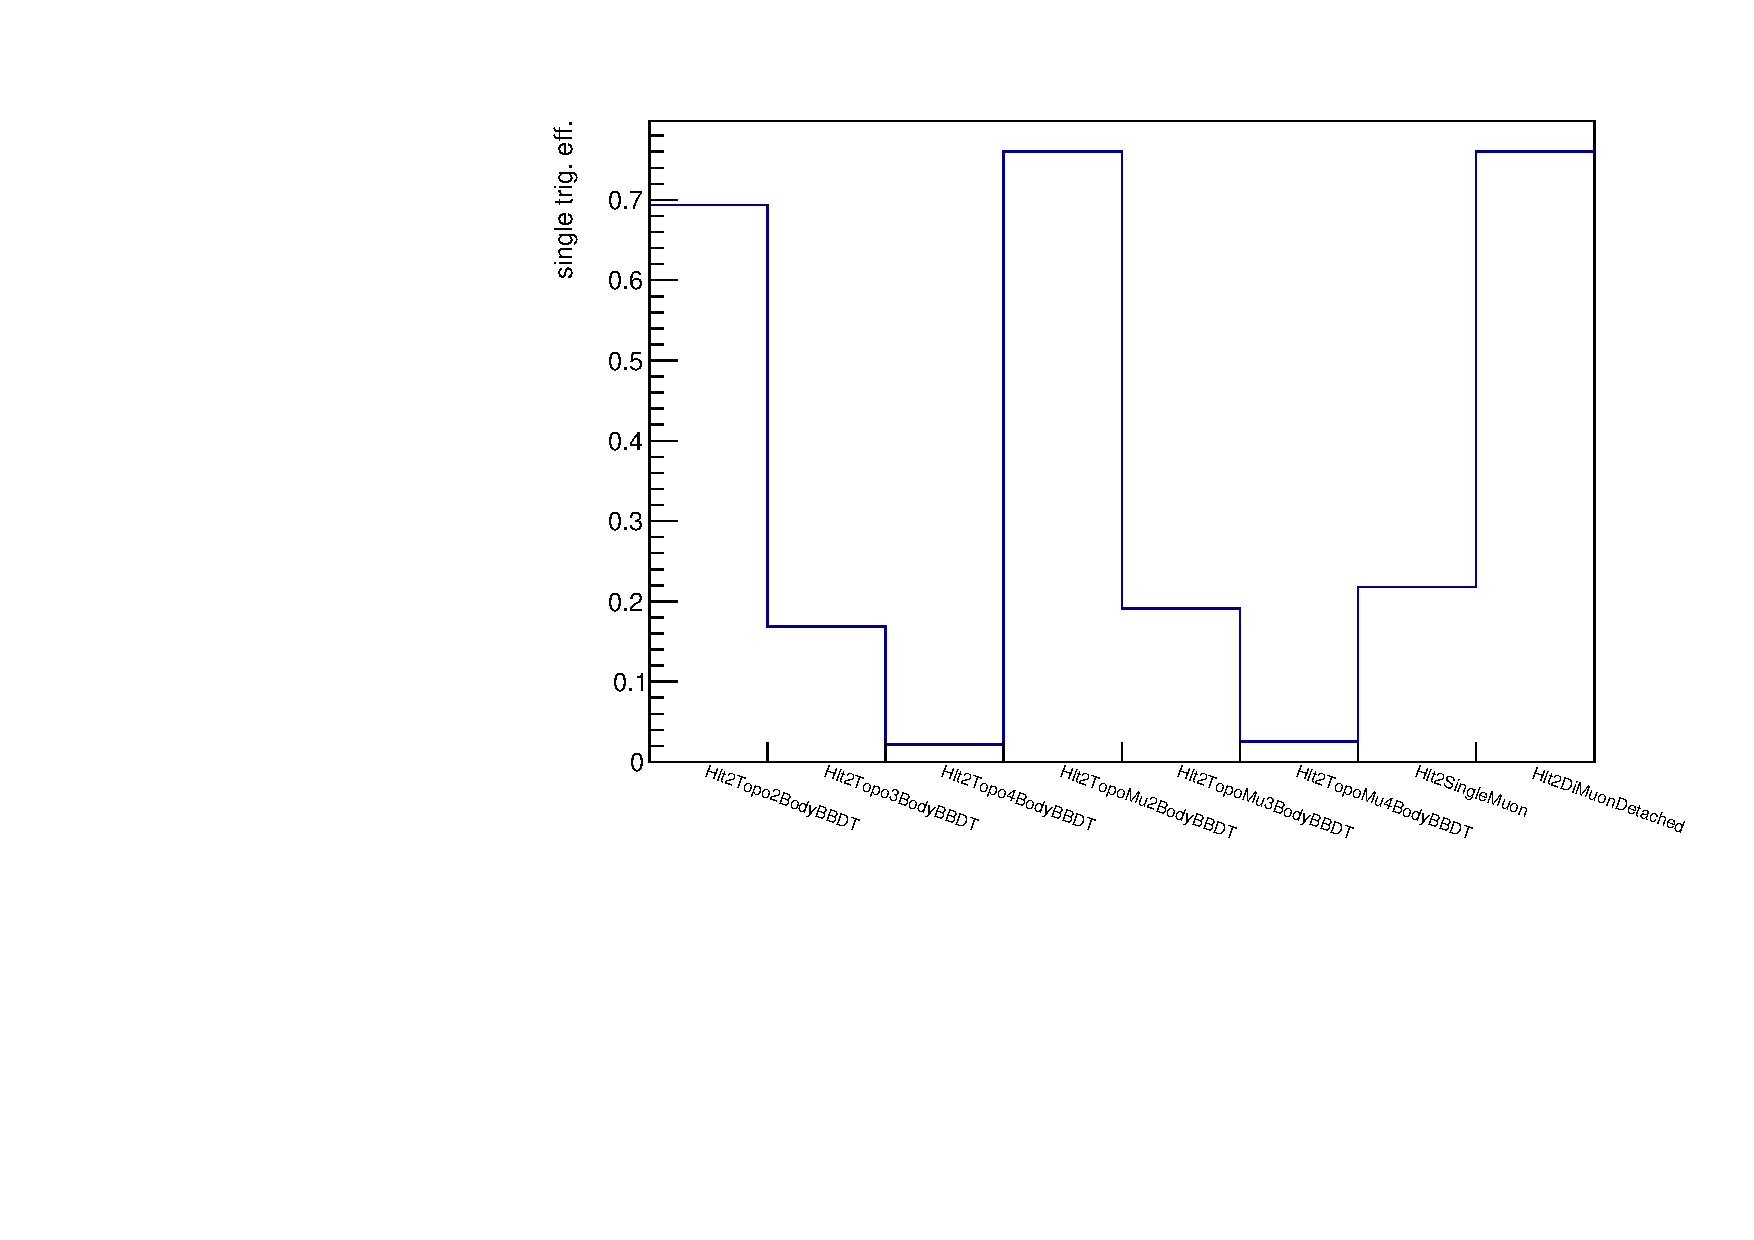
\includegraphics[width=0.48\textwidth]{Lmumu/figs/trig_highq2.pdf}
%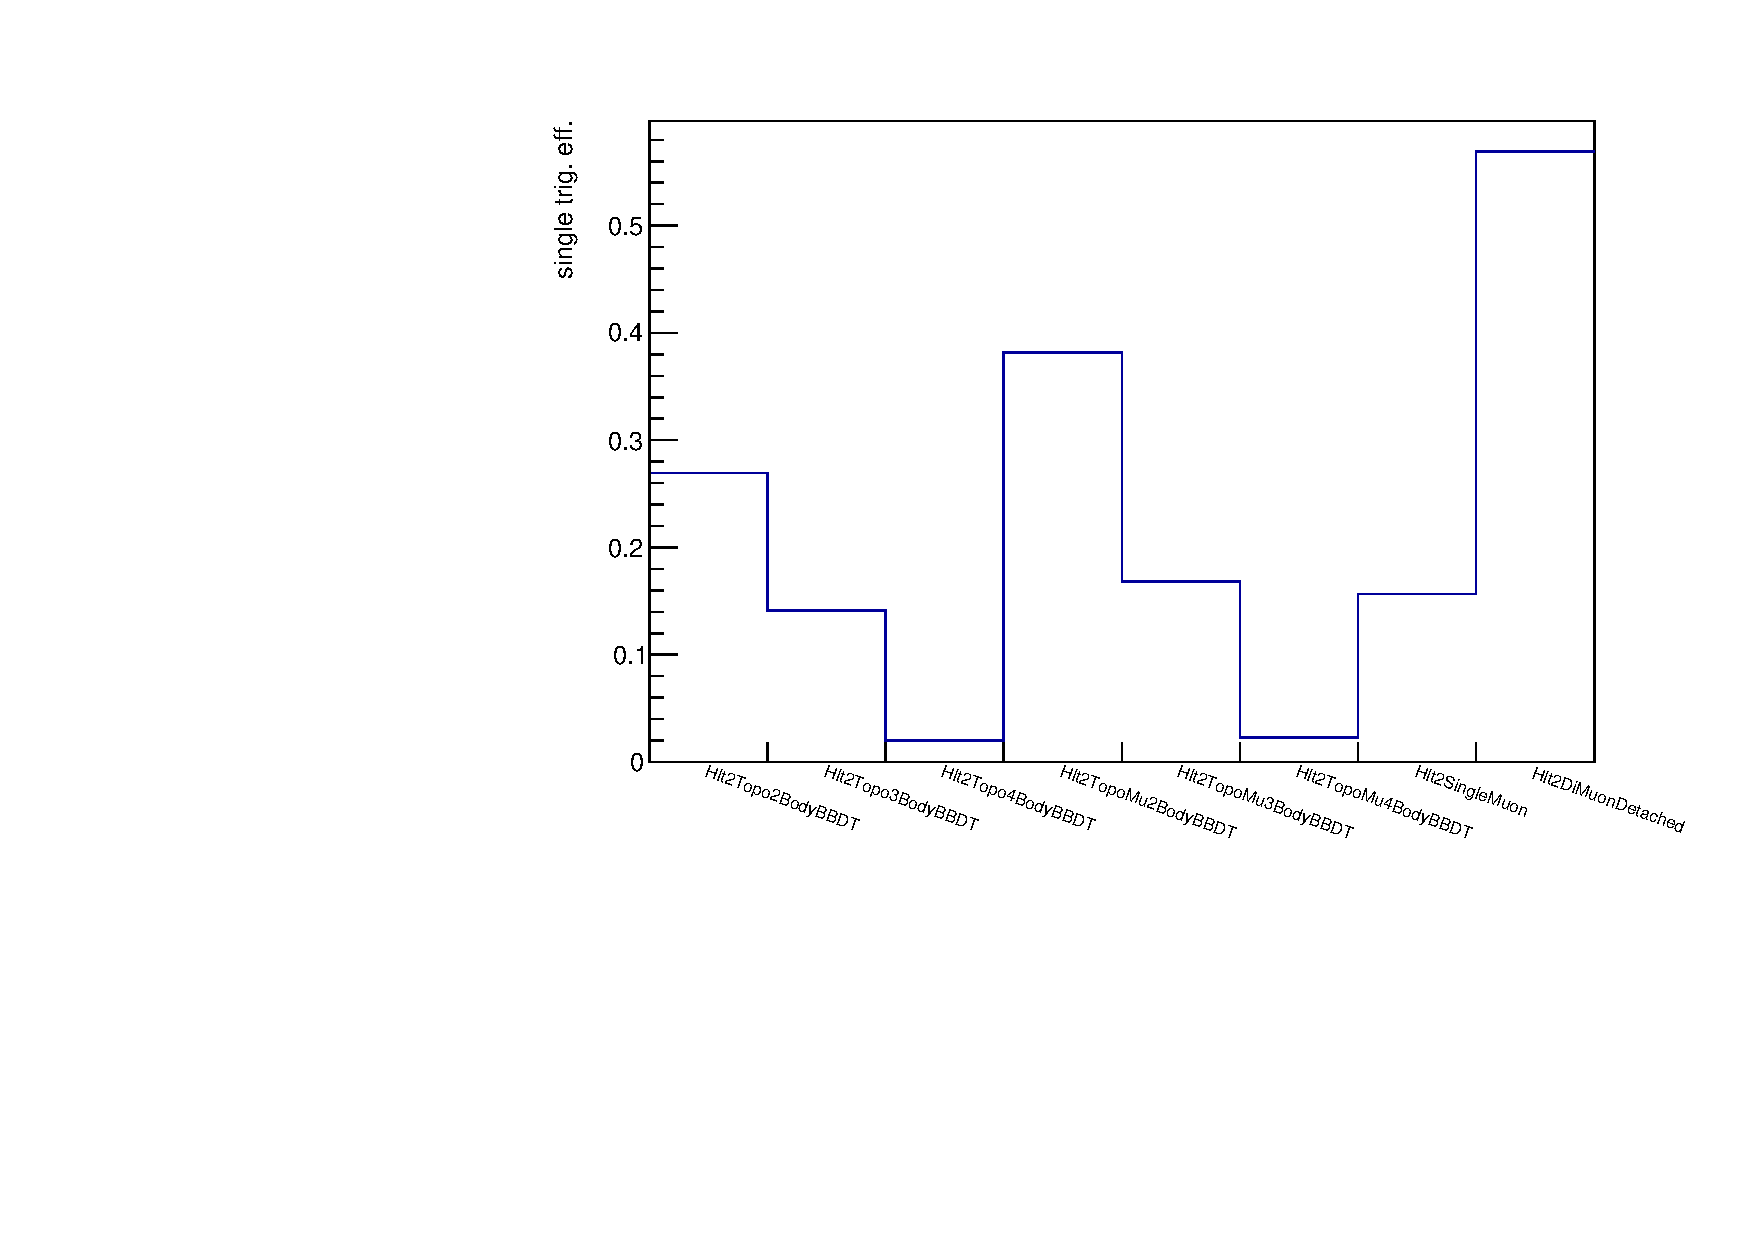
\includegraphics[width=0.48\textwidth]{Lmumu/figs/trig_lowq2.pdf}
%\caption{ Single trigger efficiency for high \qsq events (left) and low \qsq (right). }
%\label{fig:trigContrib}
%\end{figure}


\subsection{Background from specific decays}

Candidates from other decays can be reconstructed as the decays of interest if
particles are not reconstructed of mis-identified.
A survey of possible backgrounds concluded that the only physics background
to take into account comes from misreconstructed decays of \Bz to \KS with
two muons in the final state, whether via \jpsi or not, where the \KS is reconstructed 
as a \Lz with a $p\rightarrow \pi$ identity swap.
% and $m(p\pi)$ in the \Lz mass window. 
The lack of background from other decays is
mainly due to the particular topology of the \Lz decay, which is long-lived and decays at a displaced vertex.
To study the effect of misreconstructed $\Bz\ra\jpsi\KS$ and $\Bz\ra\KS\mumu$ decays
simulated samples are used. On data the $\Bz\ra\jpsi\KS$ contribution is clearly visible in the resonant channel mass distribution.
This background is not suppressed with specific cuts in this analysis as its mass shape is sufficiently distinct
the from \Lb signal and its contribution can be reliably modelled in the mass fits (see Sec.~\ref{sec:Lb_fit}).
For the rare case a rough estimate of the \KS background size is obtained using the yield in the resonant channel
rescaled by the measured ratio between the rare and resonant branching fractions.
Details are given in Sec.~\ref{sec:Lb_fit} and numbers of events predicted are reported in Tab.~\ref{tab:KSprediction}.
This contribution, although close to negligible is again considered in the fit.
A possible pollution due to $B^{+} \ra\mumu K^{*+}$ decays, where the $K^{*+}$
further decays into $\KS\pi$ is also investigated using a dedicated simulated sample and found to be negligible.
Finally, \Lb\ra\jpsi\Lz events radiating photons from the final state, can escape the \jpsi veto
and be reconstructed in the rare channel sample. Analysing simulated events it was found that the only
contribution is in the closest \qsq interval to the \jpsi tail, $6 < \qsq < 8$~\gevgevcccc.
In this interval 1.3\% of the $\Lb\to\jpsi\Lz$ candidates are reconstructed but only 0.06\%
fall into the 4-body invariant mass window used for the fits. This corresponds to $\sim 6$
events, 4 of which in the downstream category. Given the low yield and that these events do
not peak under the signal but show a decaying distribution at the edge of the fit mass window, this
background is considered as absorbed in the combinatorial background.
%Given that this contribution does not contribute in the region where we expect \Lb peak, we do
%not attempt to exclude this but it is again modelled in the fit.
Figure~\ref{fig:peakingBkgs} shows the invariant mass distribution of simulated $\Lb\ra\jpsi\Lz$
events falling into the rare \qsq region and the distribution of simulated $B^{+} \ra\mumu K^{*+}$
events mis-reconstructed as $\Lb\ra\jpsi\Lz$ decays.
%
\begin{figure}
\centering
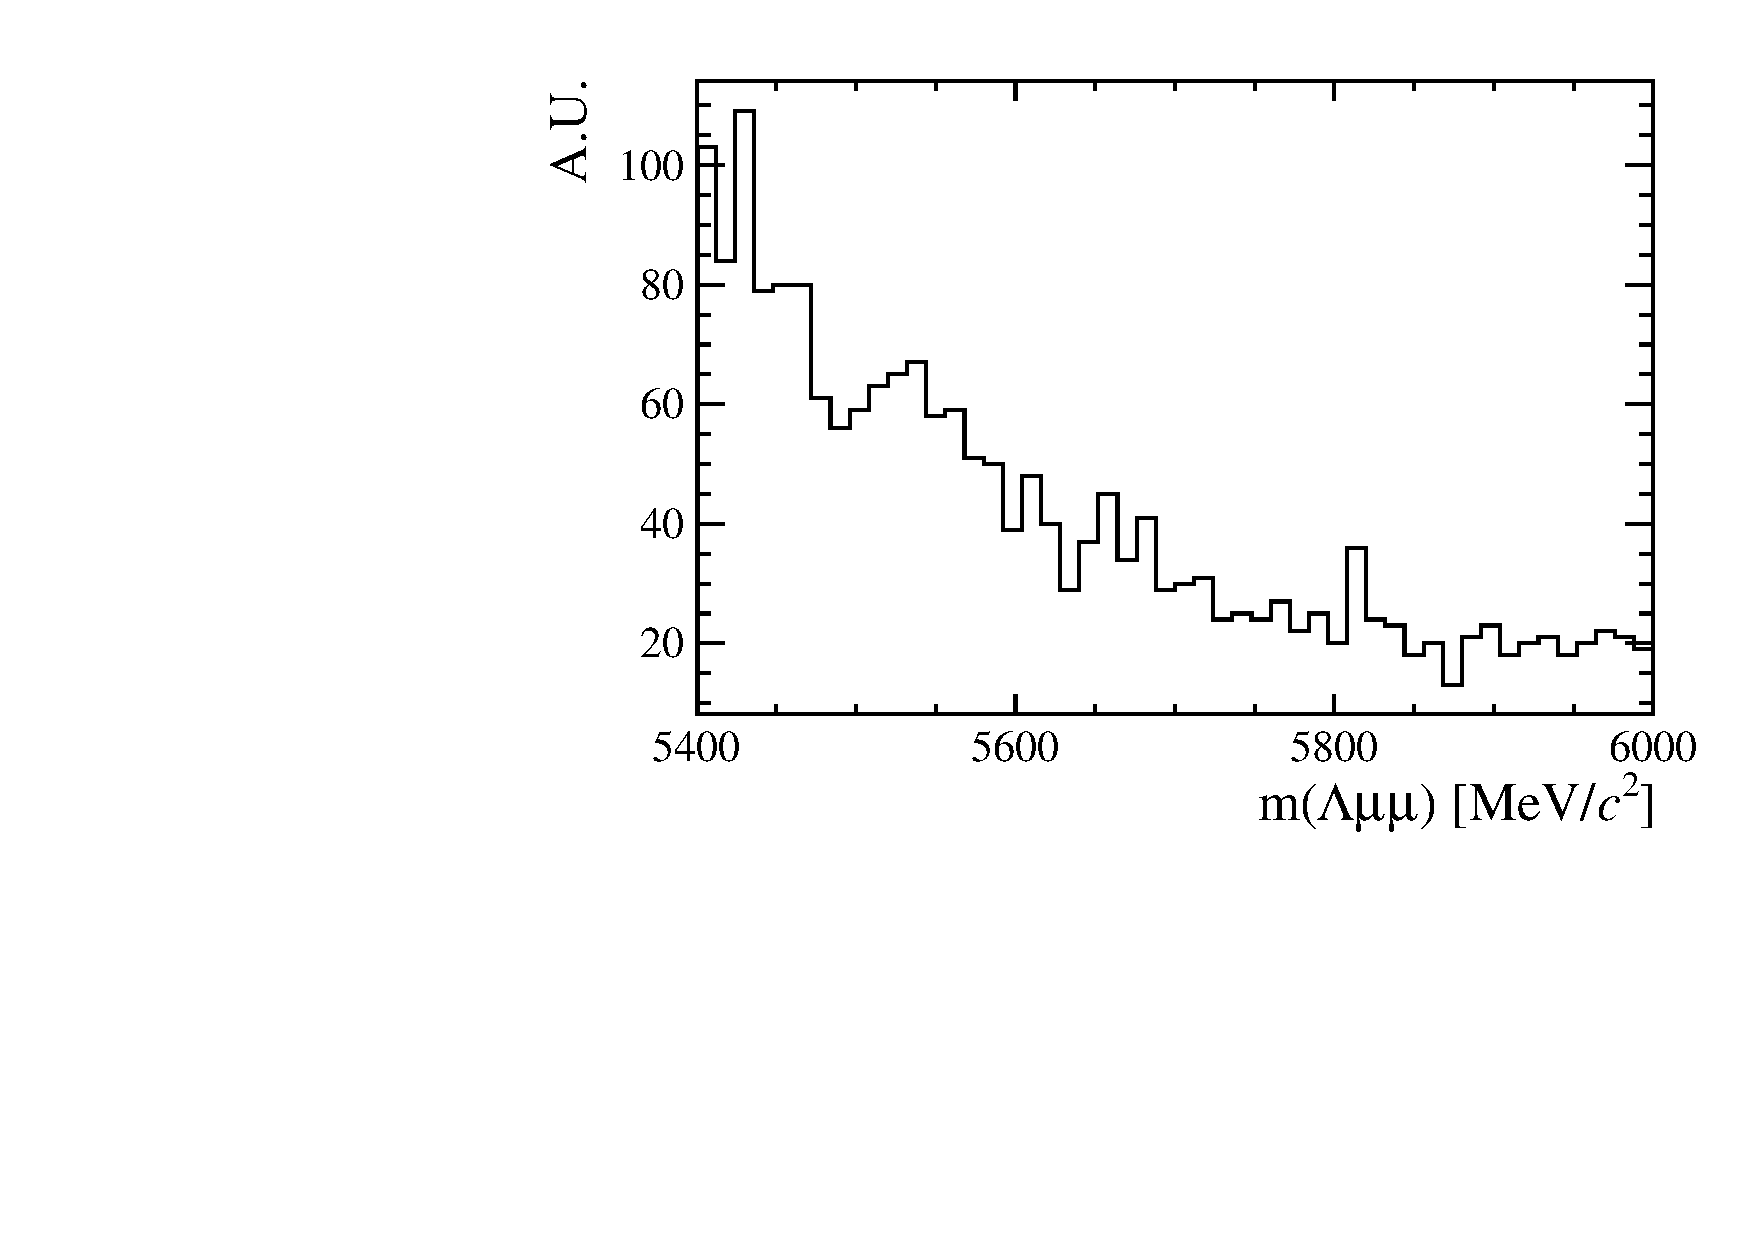
\includegraphics[width=0.49\textwidth]{Lmumu/figs/Bu2Kstplus_mass.pdf}
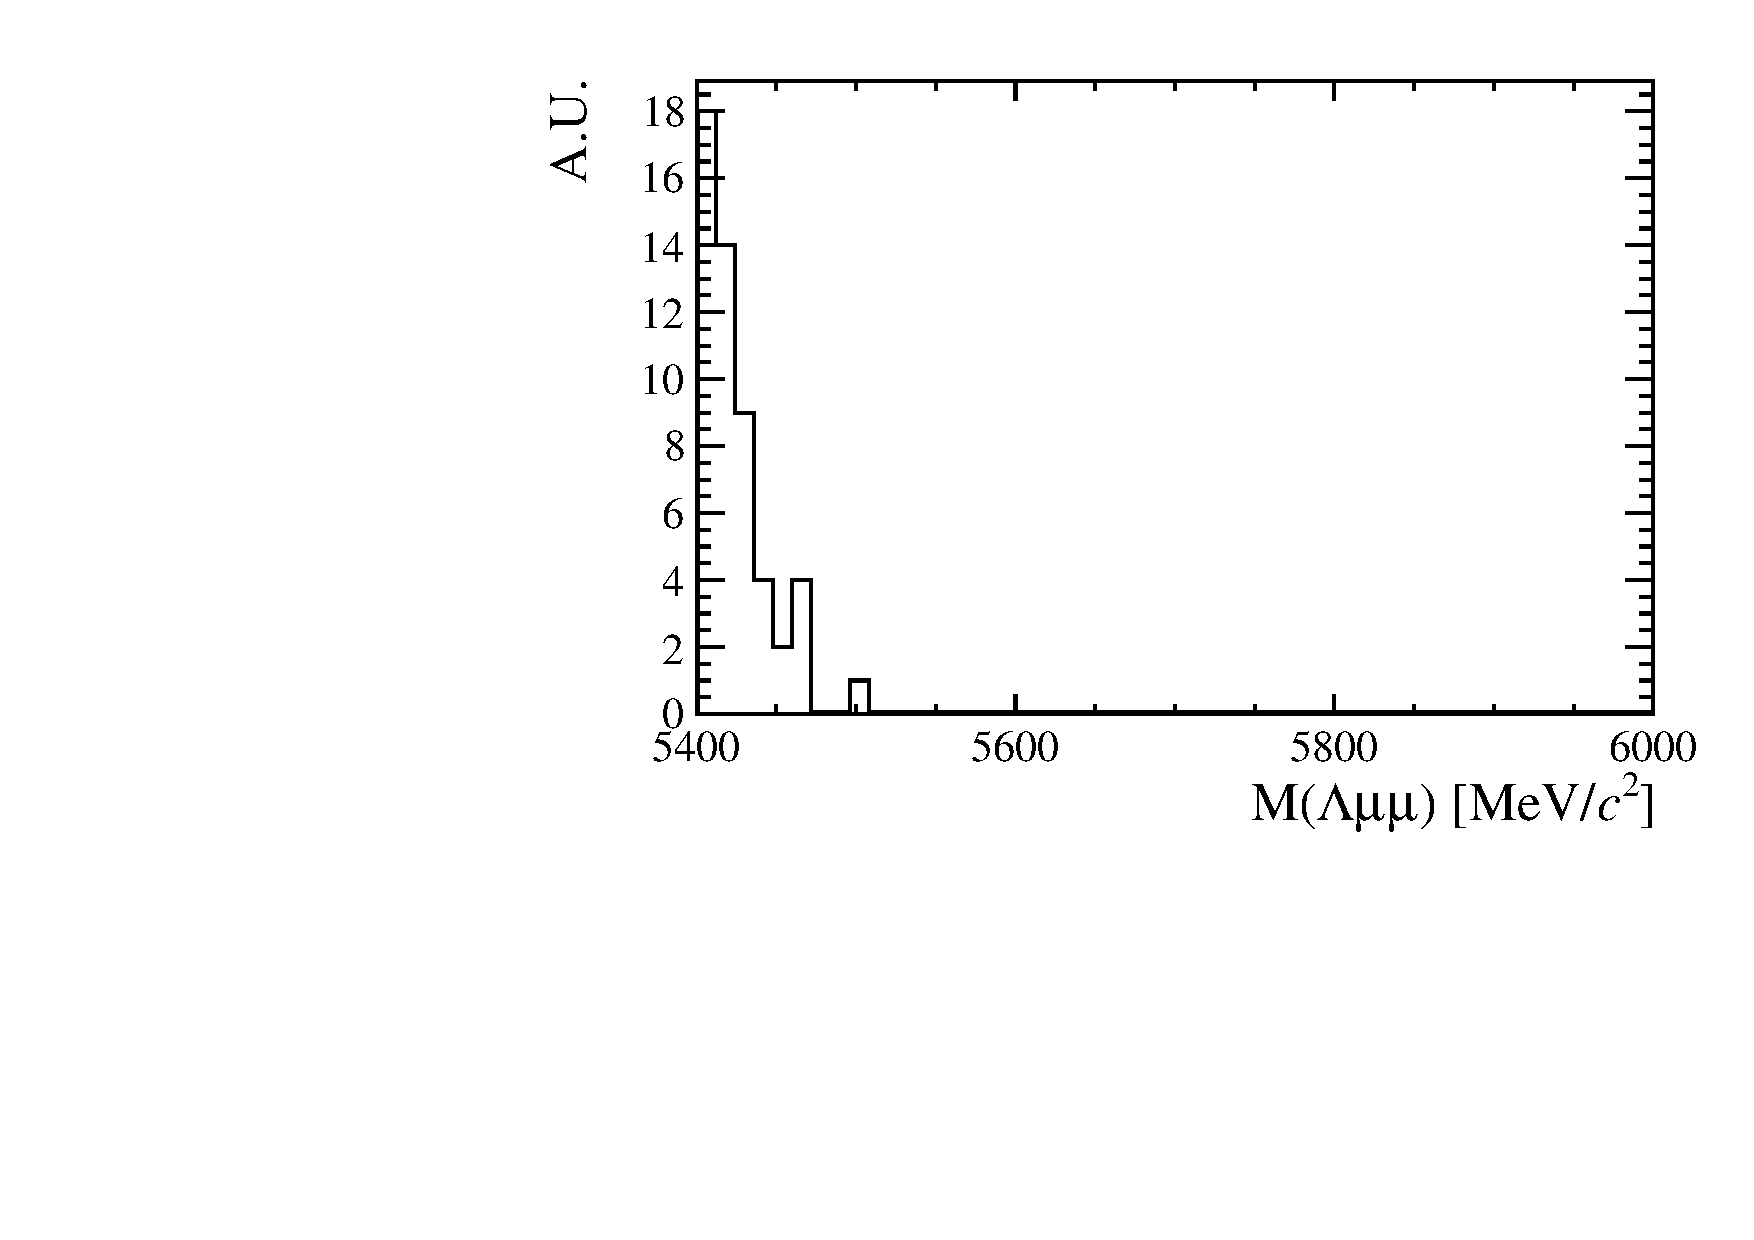
\includegraphics[width=0.49\textwidth]{Lmumu/figs/JpsiL_leakage_mass.pdf}
\caption{ Invariant mass distributions of simulated $B^{+} \ra\mumu K^{*+}$ (left)
and \Lb\to\jpsi\Lz (right) candidates passing the full selection. Only \Lb\to\jpsi\Lz
candidates reconstructed in $\qsq < 8$ \gevgevcccc are selected.
Distributions are shown in the invariant mass range relevant for the analysis 
(see Sec.~\ref{sec:Lb_fit}). }
\label{fig:peakingBkgs}
\end{figure}

